\documentclass[12pt,twoside]{report}

% some definitions for the title page
\newcommand{\reporttitle}{A Virtual Volumetric Screen}
\newcommand{\reportauthor}{Robert Buxton}
\newcommand{\supervisor}{Dr Nicole Salomons}
\newcommand{\reporttype}{MEng Individual Project}
\newcommand{\degreetype}{Computing MEng}  

% load some definitions and default packages
\input{inputs/includes}

% load some macros
% Here, you can define your own macros. Some examples are given below.

% \newcommand{\R}[0]{\mathds{R}} % real numbers
% \newcommand{\Z}[0]{\mathds{Z}} % integers
% \newcommand{\N}[0]{\mathds{N}} % natural numbers
% \newcommand{\C}[0]{\mathds{C}} % complex numbers
% \renewcommand{\vec}[1]{{\boldsymbol{{#1}}}} % vector
% \newcommand{\mat}[1]{{\boldsymbol{{#1}}}} % matrix

\newcommand{\tocite}{{\color{red} \small ToCite }} % placeholder for later citation
\newcommand{\todo}{{\color{red} \small TODO }} % placeholder for later citation

\lstdefinestyle{tree}{
literate=
  {├}{{\smash{\raisebox{-1ex}{\rule{1pt}{\baselineskip}}}\raisebox{0.5ex}{\rule{1ex}{1pt}}}}1
{─}{{\raisebox{0.5ex}{\rule{1.5ex}{1pt}}}}1
{└}{{\smash{\raisebox{0.5ex}{\rule{1pt}{\dimexpr\baselineskip-1.5ex}}}\raisebox{0.5ex}{\rule{1ex}{1pt}}}}1
}

\newcommand{\nixstore}[2][1]{\textcolor{Purple}{\texttt{/nix/store/}}\textcolor{RoyalBlue}{\texttt{#1}-}\textcolor{Orange}{\texttt{#2}}}

\newcommand{\mynewminted}[3]{%
  \newminted[#1]{#2}{#3}%
  \tcbset{myminted/#1/.style={minted language=#2,minted options={#3}}}}


%Programming Languages
\mynewminted{nix}{nix}{
  breaklines,
  linenos,
  autogobble,
  numbersep=2mm,
  fontsize=\footnotesize,
  frame=none}

\mynewminted{cpp}{cpp}{
  breaklines,
  linenos,
  autogobble,
  numbersep=2mm,
  fontsize=\footnotesize,
  frame=none}

\mynewminted{shell}{shell}{
  breaklines,
  autogobble,
  fontsize=\footnotesize,
  frame=none}


\newtcbinputlisting[auto counter,number within=section,list inside=mypyg]{\codeBoxFile}[4][]{%
  center,
  listing engine=minted,
  listing only,
  title={{\color{Black} \textbf{Listing \thetcbcounter:}} #4},
  % list entry={\protect\numberline{\thetcbcounter}#3},
  listing file={#3},
  enhanced jigsaw,
  breakable,
  colframe = Apricot!25,
  colback  = Apricot!10,
  coltitle = Apricot!20!black,
  drop fuzzy shadow,
  before skip = 20pt,
  after skip = 20pt,
  myminted/#2,
  #1}

%Boxes
\newtcolorbox[auto counter,number within=section]{figureBox}[2][]
{
  center,
  enhanced jigsaw,
  breakable,
  colframe = Apricot!25,
  colback  = Apricot!10,
  coltitle = Apricot!20!black,
  drop fuzzy shadow,
  title    = {{\color{Black} \textbf{Figure \thetcbcounter:}} #2},
  before skip = 20pt,
  after skip = 20pt,
  before upper={\centering \color{Gray!20!black}},
  #1,
}

\newtcbox[auto counter,number within=section]{\pictureBox}[2][]
{
  enhanced jigsaw,
  breakable,
  colframe = Apricot!25,
  colback  = Apricot!10,
  coltitle = Apricot!20!black,
  drop fuzzy shadow,
  title    = {{\color{Black} \textbf{Figure \thetcbcounter:}} #2},
  before skip = 20pt,
  after skip = 20pt,
  #1,
}



% load title page
\begin{document}
% !TEX root = ./main.tex

% Last modification: 2015-08-17 (Marc Deisenroth)
\begin{titlepage}

\newcommand{\HRule}{\rule{\linewidth}{0.5mm}} % Defines a new command for the horizontal lines, change thickness here

%----------------------------------------------------------------------------------------
%	LOGO SECTION
%----------------------------------------------------------------------------------------

\includegraphics[width = 7cm]{./title/figures/imperial3.png}\\[0.25cm] 

\center % Center everything on the page
 
%----------------------------------------------------------------------------------------
%	HEADING SECTIONS
%----------------------------------------------------------------------------------------

\textsc{\LARGE \reporttype}\\[0.5cm] 
\textsc{\Large Department of Computing}\\[0.5cm] 
\textsc{\large Imperial College of Science, Technology and Medicine}\\[0.5cm] 

%----------------------------------------------------------------------------------------
%	TITLE SECTION
%----------------------------------------------------------------------------------------

\HRule \\[0.4cm]
{ \huge \bfseries \reporttitle}\\ % Title of your document
\HRule \\[0.5cm]
 
%----------------------------------------------------------------------------------------
%	AUTHOR SECTION
%----------------------------------------------------------------------------------------

\begin{minipage}{0.45\textwidth}
	\begin{flushleft} \large
	\emph{Author:}\\
	\reportauthor % Your name
	\end{flushleft}
\end{minipage}
	\hfill
\begin{minipage}{0.26\textwidth}
	\begin{flushright} \large
	\emph{Supervisor:} \\
	\supervisor % Supervisor's Name
\end{flushright}
\end{minipage}
	\hfill
\begin{minipage}{0.26\textwidth}
	\begin{flushright} \large
	\emph{Second Marker:} \\
	Dr Basaran Kocer
	\end{flushright}
\end{minipage}\\[0.5cm]
	

%----------------------------------------------------------------------------------------
%	DATE SECTION
%----------------------------------------------------------------------------------------

% \includegraphics[]{./title/figures/ethics}
\adjustbox{height=10.5cm, keepaspectratio}{
	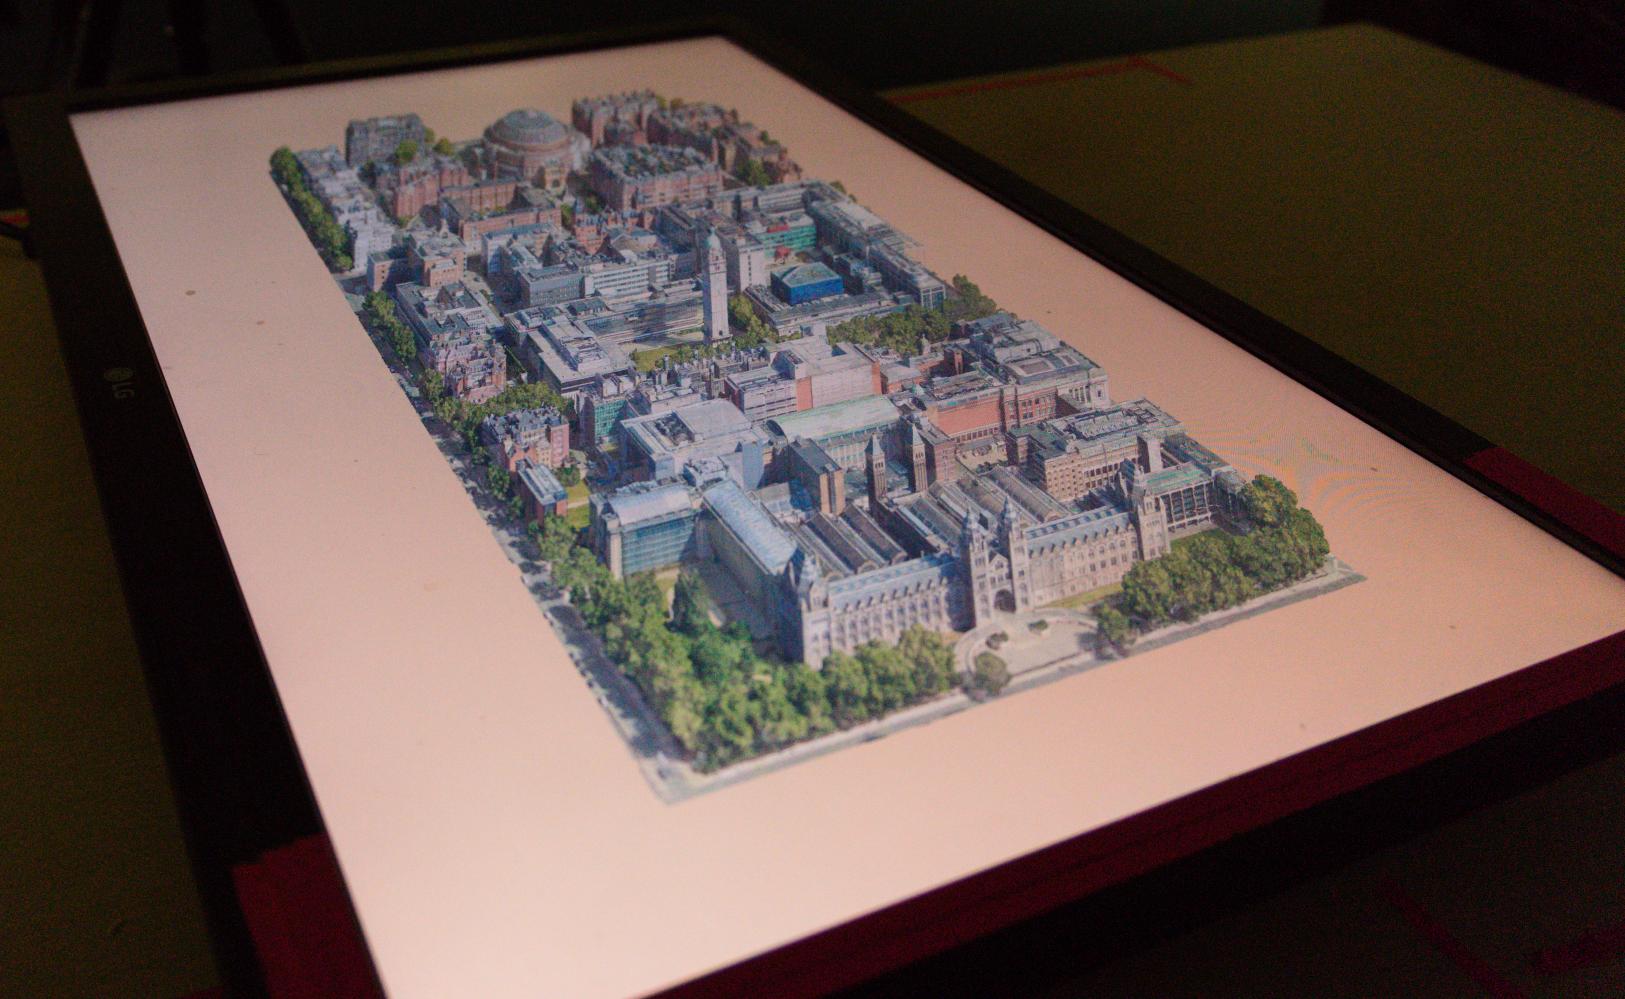
\includegraphics{./title/figures/imperial.png}
  } \\[1cm]
{\large \today} % Date, change the \today to a set date if you want to be precise


\vfill % Fill the rest of the page with whitespace
Submitted in partial fulfillment of the requirements for the \degreetype~of Imperial College London

\end{titlepage}



% page numbering etc.
\pagenumbering{roman}
\clearpage{\pagestyle{empty}\cleardoublepage}
\setcounter{page}{1}
\pagestyle{fancy}

% %%%%%%%%%%%%%%%%%%%%%%%%%%%%%%%%%%%%
\begin{abstract}
	This thesis presents the development of a virtual volumetric screen designed to simulate volumetric displays for Human-Computer Interaction (HCI) research. The primary objective is to create a cost-effective, reproducible, and simple system that enables researchers to explore the usability of volumetric displays without requiring access to expensive and specialized hardware. The system employs head and hand tracking to render 3D content on a standard 2D monitor, creating the illusion of depth and allowing natural interaction with virtual objects. \\
	
	A comprehensive user study was conducted to evaluate the effectiveness of the system. The study compared user performance in tasks requiring spatial interaction under different conditions: 3D versus 2D views and direct hand interaction versus teleoperation. The results showed a significant improvement in task performance when using a 3D view with direct hand interaction, highlighting the importance of intuitive and immersive interaction modes in volumetric display research. \\
	
	Future work includes expanding the system's compatibility with different hardware and operating systems, improving hand tracking accuracy, and exploring multi-user support. 
\end{abstract}

% \cleardoublepage
% %%%%%%%%%%%%%%%%%%%%%%%%%%%%%%%%%%%%
\section*{Acknowledgments}
I would like to thank \textbf{in order of importance}:
\begin{itemize}[noitemsep]
	% \item ChatGPT
    \item My supervisor Dr Nicole Salomons for her guidance and support throughout this project so far.
    \item My loving family who still think I am studying physics (\textbf{Mabel}) for some reason.
\end{itemize}
\clearpage{\pagestyle{empty}\clearpage}

%%%%%%%%%%%%%%%%%%%%%%%%%%%%%%%%%%%%
%--- table of contents
\fancyhead[RE,LO]{\sffamily {Table of Contents}}
\tableofcontents


\clearpage{\pagestyle{empty}\clearpage}
\pagenumbering{arabic}
\setcounter{page}{1}
\fancyhead[LE,RO]{\slshape \rightmark}
\fancyhead[LO,RE]{\slshape \leftmark}

%%%%%%%%%%%%%%%%%%%%%%%%%%%%%%%%%%%%
\chapter{Introduction}
\section{Motivations}
A volumetric display is a type of graphical display device that can provide a visual representation of objects natively in 3D. They can be viewed from any angle without the need for special visual apparatus by multiple people simultaneously \cite{1492264}. These displays differ from more traditional virtual reality devices in that they are not immersive, but rather they are a window into a virtual world (See Fig~\ref{fig:passive-optical} and Fig~\ref{fig:acoustic}). There is no real consensus on what exactly constitutes a volumetric display, let alone the best way to build one. As we cover in the background section there are currently many different approaches being attempted by research groups both academic and industrial to create these displays. 
 
\begin{invisBox}
\pictureBox[label={fig:passive-optical}]{One of Columbia University's passive optical scattering based volumetric displays \cite{10.1145/1179849.1179982}}{
  \adjustbox{height=5.0cm, keepaspectratio}{
    \includegraphics{./introduction/figures/passive optical scatterers.png}
  }
}
\hfill
\pictureBox[label={fig:acoustic}]{One ofBristol University's acoustic trapping based volumetric displays \cite{10.1063/1.5113467}}{
\adjustbox{height=5.5cm, keepaspectratio}{
  \includegraphics{./introduction/figures/acoustophoretic display.jpg}
  }
}
\end{invisBox}

At the time of writing it is difficult to conduct human-computer interaction (HCI) research into the field of volumetric displays because these devices are not widely available, expensive and difficult to manufacture, and have extreme bandwidth requirements which makes it difficult to conduct user studies and experiments. People have created virtual simulations of volumetric displays before to try and solve this problem, but these solutions are often complicated and expensive to replicate.

\section{Objectives}

With the conclusion of this project, we aim to produce a cheap, multi-platform, lightweight and simple platform for simulating volumetric displays through the use of a Fish tank virtual reality (FTVR) device (See background). We hope that this will reduce the barrier to entry for researchers who wish to conduct HCI research in the field of volumetric displays. We aim to make the following contributions:
\subsection{Volumetric Simulator}
We plan to create a platform for simulating volumetric displays that is:
\begin{itemize}
  \item \textbf{Multi-platform}: We have packaged our platform in the Nix package manager \cite{dolstra2004nix} which allows it to be easily run and ported to any platform and hardware that Nix supports.

  \item \textbf{Lightweight}: We use simple rending algorithms in OpenGL \cite{rost2009opengl} to create our virtual volumetric display allowing our software to be computationally cheap to run compared to more fully-fledged rendering/games engines that might be used typically for HCI research like Unity.

  \item \textbf{Cheap}: By relying on only a generic depth camera and a standard display our software requires minimal hardware to run, making research conducted on our platform cheap and easy to run.

  \item \textbf{Reproducible:} By building with Nix we can guarantee that any experiments conducted using this platform will be completely reproducible. (See background)
\end{itemize}

\subsection{User experiment}
We plan to conduct an HCI user study to demonstrate the utility of our volumetric display simulation platform. We will conduct the user study to compare the relative effectiveness of using hand tracking to interact directly with an ethereal/incorporeal volumetric display compared to a via teleoperation with a corporeal/tangible display (See evaluation).


%%%%%%%%%%%%%%%%%%%%%%%%%%%%%%%%%%%%
\chapter{Ethical Discussion}
\section{User Study}
\begin{enumerate}
	\item Got ethical approval from ethics committee. 
\end{enumerate}
\label{sect:ethics}

%%%%%%%%%%%%%%%%%%%%%%%%%%%%%%%%%%%%
\chapter{Background}
\section{Volumetric displays}

Volumetric displays \cite{1492264} are a promising technology that offers a captivating three-dimensional viewing experience. By emitting light for each voxel, or volume element, in a 3D space, these displays transcend the limitations of traditional 2D planes, providing a truly immersive 3D effect. This innovative approach enables the accurate representation of virtual 3D objects, including focal depth, motion parallax, and vergence, which refers to the rotation of a viewer's eye to fixate on the same point they are focusing on. Moreover, volumetric displays allow multiple users to view the same display from different angles, providing unique perspectives of the same object.

\subsection{Swept Volume Displays}
Swept volume displays represent one category of volumetric displays. They employ a moving 2D display to create a 3D image. This is achieved by moving the 2D display through a 3D space and emitting light from the display at each point. Common techniques for achieving this includes using a rotating mirror \cite{10.1117/12.480930}, emitting screen typically an LED \cite{Gately:11}, or transparent projector screen \cite{keane_volumetric_2016}. There currently exist commercial products that implement this as can be seen in Fig~\ref{fig:swept-volume-displays}.

\begin{figureBox}[label={fig:swept-volume-displays}]{Two different types of swept volume display}
  \begin{minipage}[t]{0.48\textwidth}
    \includegraphics[width=\textwidth]{./background/figures/3d/voxon.jpg}
    \small {a) The VXR4612 3D Volumetric Display, a projector based persistence of vision display produced by Voxon Photonics. \tocite}
  \end{minipage}\hfill
  \begin{minipage}[t]{0.48\textwidth}
    \includegraphics[width=\textwidth]{./background/figures/3d/brightvox.png}
    \small {b) A Volumetric Display / Holographic Signage, a LED based persistence of vision display produced by Brightvox Inc. \tocite}
  \end{minipage}
\end{figureBox}

\subsection{Static Volume Displays}
Static volume displays are another category of volumetric displays. They employ a static 3D display to create a 3D image. This is achieved by emitting light from the display at each point in a 3D space. Techniques for achieving this range from using a 3D array of LEDs \cite{10.1145/2341931.2341937}, lasers and phosphorus gas \cite{https://doi.org/10.1002/anie.202003160}, or a transparent laser induced damaged medium that can be projected into \cite{10.1145/1179849.1179982}.

\subsection{Trapped Particle displays}
{\textcolor{red}{TODO}}

\subsection{Photon displays}
{\textcolor{red}{TODO}}

\subsection{Issues}

Expensive: Swept volume displays require extremely high refresh rate projectors, which are expensive and difficult to manufacture or transparent LED screens which are only recently becoming widely available. For example the Voxon VX1 one of the few if only commercial available volumetric displays costs \$11,700 USD \cite{noauthor_products_nodate}. \\

High bandwidth requirements: To render objects in real time at 2D display equivalent resolutions while taking a raw voxel stream (as apposed to calculating voxels on hardware from primitive shapes) has an extremely high bandwidth requirement. \texttt{60fps} on a $4096 \times 2160 \times 1080$ voxel display with \texttt{24 bit} color requires a bandwidth of $1.37 \times 10^3$ bits per second/13.7 terabits per second. To achieve that currently would require about 170 state-of-the-art Ultra High Bit Rate (UHBR) (80 gigabit) DisplayPort cables simultaneously. It was predicted in 2021 \cite{LAM2021050011} that a based on the historical trend of display bandwidth that a volumetric 4K screen will become feasible in 2060.

\subsection{Volumetric Screen Simulations}
Because of the high cost and bandwidth requirements of volumetric displays, there has been some research into simulating volumetric displays on traditional 2D displays. One commonly used method is the so called fish tank virtual reality (FTVR) display \cite{10.1145/3290605.3300763} \cite{Zabarauskas2012}
\label{sect:3d}
\section{Nix/NixOS}

\begin{figureBox}[label={fig:nix-snowflake}]{the NixOS logo, also know as the Nix Snowflake.}
  \includegraphics[width=0.2\linewidth]{./figures/background/nix/nix-snowflake.pdf}
\end{figureBox}

\textbf{Nix} \cite{dolstra2004nix} is an open-source, "purely functional package manager” used in unix-like operating systems to provide a functional and reproducible approach to package management. Started in 2003 as research project Nix \cite{dolstra2006purely} is widely used in both industry \cite{NixCommunityNixOSWiki} and academia \cite{10.1145/3152493.3152556} \cite{https://doi.org/10.1002/qua.26872} \cite{LHCbNix}, and its associated public package repository \texttt{nixpkgs} \cite{NixPkgs} as of Jan 2024 has over 80,000 unique packages making it the largest up-to-date package repository in the world as can be seen in Fig~\ref{fig:package-manager-comparison}. Out of Nix has also grown \textbf{NixOS} \cite{10.1145/1411204.1411255} \label{nix-snowflake} a Linux distribution that is conceived and defined as a deterministic and reproducible entity that is declared functionally and is built using the \textbf{Nix} package manager. \\

%% Repology Package Manager Comparison
\begin{figureBox}[label = {fig:package-manager-comparison}]{Comparison of all package repositories from Repology.org \cite{Marakasov_2024}}
\fontsize{5}{6}\selectfont
\includegraphics[width=\linewidth]{./figures/background/nix/pkg-compare.pdf}
\end{figureBox}

Nix packages are defined in the \textbf{Nix Language} a lazy functional programming language where packages are treated like purely functional values that are built by side effect-less functions and once produced are immutable. Packages are built with every dependency all the way down to the \texttt{ELF} interpreter and \texttt{libc} (C standard library) defined in nix. All packages are installed in the store directory, typically \texttt{/nix/store/} by their unique hash and package name as can be seen in Fig~\ref{fig:nix-store-path}.

%% Nix Store Path
\begin{figureBox}[label={fig:nix-store-path}]{Nix Store Path}
\begin{tabbing}
\={\color{Purple}\texttt{/nix/store/}}\={\color{RoyalBlue}\texttt{sbldylj3clbkc0aqvjjzfa6slp4zdvlj}}-\={\color{Orange}\texttt{hello-2.12.1}} \\
\>\small{Prefix} \>\small {Hash part} \>\small {Package name}
\end{tabbing}
\end{figureBox}

Source files, like tarballs and patches are downloaded and stored in the store directory to insure all required inputs are always available. As different dependencies result in a different hash and therefore location in the store directory you can have multiple versions or variants of the same package installed while also at the same time avoiding "DLL hell" by making it impossible to accidentally point at the wrong package. Another important result is that upgrading or uninstalling a package cannot ever break other applications. Nix builds packages in a sandbox to ensure packages are built the same way on every machine by restricting access to non reproducible files and the network \cite{nixcon-sandboxs}. A package can be pinned (and should be) to nix release meaning that once it builds and works today it will continue to work the exact same way in the future, regardless of when and where it is used. \\ 


These features provide extremely useful for scientific work, CERN uses Nix to package the LHCb Experiment because it allows software to be stable for long periods of time (longer than ever long term support operating systems) and it means that as the software is reproducible; all the experiments are completely reproducible as all bugs present in the original version stay to ensure the accuracy of the results \cite{LHCbNix}. \\


To create a package Nix evaluates a \textbf{derivation} which is a specification/recipe that defines how a package should be built. It includes all the necessary information and instructions for building a package from its source code, such as the source location, build dependencies, build commands, and post-installation steps. By default, Nix uses binary caching to build packages faster, the default cache is \texttt{cache.nixos.org} is open to everyone and is constantly populated by CI systems. You can also specific custom caches. The basic process for building nix packages can be seen in Fig~\ref{fig:nix-derivation-loop}.

\begin{figureBox}[label = {fig:nix-derivation-loop}]{Nix Build Loop}
\begin{enumerate}
    \item A hash is computed for the derivation and, using that hash, generate a nix store path, e.g \nixstore[sbldylj3clbkc0aqvjjzfa6slp4zdvlj]{hello-2.12.1}.
    \item  With the store path in hand, check if the derivation has already been built. First, checks the configured Nix store e.g {\color{Purple}\texttt{/nix/store/}} to see if the path e.g {\color{RoyalBlue}\texttt{sbldylj3clbkc0aqvjjzfa6slp4zdvlj}}-{\color{Orange}\texttt{hello-2.12.1}} already exists. If it does, use that it, if not continue.
    \item Next it checks if the store path exists in a configured binary cache, this is by default \texttt{cache.nixos.org}. If it does download from the cache and use that if not continue.
    \item Use Nix to build the derivation from scratch, recursively following all of the steps in this list, using already-realised packages whenever possible and building only what is necessary. 
\end{enumerate}
\end{figureBox}


\begin{codeBox}[label = {fig:nix-flake}]{nix}{flake.nix}
{
  description = "A flake for building Hello World";
  inputs.nixpkgs.url = "github:NixOS/nixpkgs/nixos-23.11";

  outputs = { self, nixpkgs }: {
    defaultPackage.x86_64-linux =
      let
        pkgs = nixpkgs.legacyPackages.x86_64-linux;
      in
      pkgs.stdenv.mkDerivation {
        name = "hello-2.12.1";
        src = self;
        # Not strictly necessary as stdenv will add gcc
        buildInputs = [ pkgs.gcc ];
        configurePhase = "echo 'int main() { printf(\"Hello World!\"); }' > hello.c";
        buildPhase = "gcc -o hello ./hello.c";
        installPhase = "mkdir -p $out/bin; install -t $out/bin hello";
      };
  };
}
\end{codeBox}

\begin{codeBox}[label = {fig:nix-terminal}]{shell}{Terminal}
[shell:~]$ ls 
flake.lock  flake.nix

[shell:~]$ nix flake show 
└──defaultPackage 
   └──x86\_64-linux: package 'hello-2.12.1'

[shell:~]$ nix run . 
Hello, world! 

[shell:~]$ tree $(nix path-info .) 
"\nix\store\sbldylj3clbkc0aqvjjzfa6slp4zdvlj-hello-2.12.1"
└──bin
   └──hello
   
[shell:~]$ TODO get nix depencies
/nix/store/s2f1sqfsdi4pmh23nfnrh42v17zsvi5y-libunistring-1.1
/nix/store/08n25j4vxyjidjf93fyc15icxwrxm2p8-libidn2-2.3.4
/nix/store/lmidwx4id2q87f4z9aj79xwb03gsmq5j-xgcc-12.3.0-libgcc
/nix/store/qn3ggz5sf3hkjs2c797xf7nan3amdxmp-glibc-2.38-27
/nix/store/sbldylj3clbkc0aqvjjzfa6slp4zdvlj-hello-2.12.1
\end{codeBox}

\begin{figureBox}{Dependency graph}
\includegraphics[width=0.5\linewidth]{./figures/background/nix/hello-pkg.pdf}
\end{figureBox}

For an example of making our own nix package. I have create a flake in Fig~ that builds the basic "hello" package also available on \texttt{nixpkgs}. \\

Highlighting particular lines in the \texttt{flake.nix} \\

\textbf{Line 2:} We have specified that we want to build our flake with the stable \textbf{nix channel} \texttt{nixos-23.11}, the most recent channel at the time of writing. This "channel" is really just a release branch on the nixpkgs github repository. Channels do receive conservative updates such as bug fixes and security patches but no major updates after initial release. The first time I build the hello package from my \texttt{flake.nix} a \texttt{flake.lock} is automatically generated that pins us to a specific revision of \texttt{nixos-23.11}. Our built inputs will not change until we relock our flake to either a different revision of \texttt{nixos-23.11} or a new channel entirely. \\

\textbf{Line 5:} Here we define \texttt{outputs} as a function that accepts, \texttt{self} (the flake) and \texttt{nixpkgs} (the set of packages we just pinned to on the line 2). What nix does is resolves all inputs and then calls the \texttt{output} function.\\

\textbf{Line 6:} Here we specify that we are defining the default package for users on \texttt{x86\_64-linux}. If we tried to build this package on a different cpu architecture like for example ARM (\texttt{aarch64-linux}) the flake would refuse to build the package  as it has not been defined for ARM yet. If we desired we could fix this by adding a \texttt{defaultPackage.aarch64-linux} definition.\\

\textbf{Line 7-9:} Here we are just defining a shorthand way to referring to x86 linux packages. This syntax is similar if not identical to Haskell.\\

\textbf{Line 10:} Here we begin the definition of the derivation which is the instruction set nix uses to build the package.\\

\textbf{Line 14:} We specify here that we need \texttt{gcc} in our sandbox to build our package. \texttt{gcc} here is shorthand for \texttt{gcc12} but we could specify and c compiler and version of that compiler we liked. If you really wanted to you could compile different parts of the code with different versions of gcc.\\

\textbf{Line 15:} Here we are slightly abusing the configure phase to generate a hello.c file. Each phase is essentially run as a bash script. Everything inside \texttt{mkDerivation} is happening inside a sandbox and will be discarded once the package is built (techically after we garbage collect). \\

\textbf{Line 16:} Here we actually build our package \\

\textbf{Line 17:} In this line we copy our executable we have generate which is currently in the sandbox into the actual package we are producing. \\ 

\label{sect:nix}

%%%%%%%%%%%%%%%%%%%%%%%%%%%%%%%%%%%%
\chapter{Methods}
\section{Perspective Projection}

\begin{figureBox}[label={fig:ortho-vs-persp}]{Orthographic and perspective projections}
    \includegraphics[width = 0.8\linewidth]{./background/figures/projection/ortho-vs-persp.pdf}
\end{figureBox}

To represent 3D objects on a 2D surface (our screen) OpenGL support two type of projections: perspective and orthographic as seen in Fig~\ref{fig:ortho-vs-persp}. Orthographic features parallel projection lines (orthogonal to the projection plane), which means that it does not depict the effect of perspective. Distances are preserved, making it useful for technical drawings where measurements need to be accurate and unskewed by perspective (All diagrams in this report are in the orthographic perspective). Unlike orthographic projection, perspective projection simulates the way the human eye perceives the world, with objects appearing smaller as they are farther from the viewpoint as the projection lines converge at a vanishing point. To create the illusion of 3D in this project we must use a perspective projection. \\

\begin{figureBox}[label={fig:persp-projection}]{Using frustum to generate a perspective projection}
    \includegraphics[width = 0.5\linewidth]{./background/figures/projection/persp-projection.pdf}
\end{figureBox}

OpenGL provides the \texttt{frustum} function as seen in Fig~\ref{fig:persp-projection} which can be used to construct a perspective matrix Fig~\ref{fig:perspective-matrix} that maps a specified viewing frustum  screen-space (with intermediate steps handelled by OpenGL) \tocite. The viewing frustum, is specified by six parameters: $f$, $l$, $r$, $b$, $t$, $n$ which represent left, right, bottom, top, near, and far. These parameters define the sides of the near clipping plane, highlighted in red, relative to the origin of the coordinate system. These parameters do not represent distances or magnitudes in a traditional sense but rather define the vectors from the center of the near clipping plane to its edges. \\

\begin{figure}[H]
    \[
        \begin{bmatrix}
            \frac{2n}{r-l} & 0              & \frac{r+l}{r-l}  & 0                \\
            0              & \frac{2n}{t-b} & \frac{t+b}{t-b}  & 0                \\
            0              & 0              & -\frac{f+n}{f-n} & -\frac{2fn}{f-n} \\
            0              & 0              & -1               & 0                \\
        \end{bmatrix}
    \]
    \caption{frustum perspective matrix}
    \label{fig:perspective-matrix}
\end{figure}

The $l$ and $r$ parameters specify the horizontal boundaries of the frustum on the near clipping plane, with left typically being a negative value and right a positive value, defining the extent to which the frustum extends to the left and right of the origin. Similarly, the $b$ and $t$ parameters determine the vertical boundaries, with bottom often negative and top positive, expressing the extent of the frustum below and above the origin. \\

The $n$ and $f$ parameters are scalar values that specify the distances from the origin to the near and far clipping planes along the view direction. Altering the value of $n$ will change the angles of the lines (or vectors) that connect the corners of the near plane to the eye, effectively changing the "field of view". Changing the value $f$ affects the range of depth that is captured within the scene. \\

If we are able to track the position of a viewers eye in real time then we can create the illusion of a 3D scene behind and in front of a display using \texttt{frustum}. This can be done fairly trivially following Robert Kooima's method he sets out in "Generalised Perspective Projection" to calculate $f$, $l$, $r$, $b$, $t$, $n$ as the viewers eye moves \cite{kooima2009generalized}. \\



To encode the position and size of the screen we take 3 points, $p_a$, $p_b$ and $p_c$ which represent the lower-left, lower-right and upper left points of the screen respectively when viewed from the front on. These points are in tracker space, the co-ordinate system of the device we use to track the eyes. These point can be used to generate an orthonormal basis of the screen of $s_r$, $s_u$ and $s_n$ which represents the directions up, right and normal to the screen respectively as seen in Fig~\ref{fig:perspective-screen}. We can compute these values from the screen corners as follows:
\[s_r = \frac{p_b-p_a}{||p_b-p_a||} \quad s_u = \frac{p_c-p_a}{||p_c-p_a||} \quad s_n = \frac{s_r\times s_u}{||s_r \times s_u||}\]

\begin{figureBox}[label={fig:perspective-screen}]{Defining a screen in 3D space}
    \includegraphics[width = 0.3\linewidth]{./background/figures/projection/screen.pdf}
\end{figureBox}

Introducing the viewers eye which we will refer to as $p_e$. We can draw three vectors $v_a$, $v_b$, $v_c$ from the viewers eye $p_e$ to the corners of the screen $p_a$, $p_b$, $p_c$ as seen in Fig~\ref{fig:screen-extents}. In the diagram we also have labelled the components of each of these vectors in the basis of the screen. We can compute these as follows:
\[ v_a = p_a - p_e \quad v_b = p_b - p_e \quad v_c = p_c - p_e\] \\

To calculate the required values for \texttt{frustum} we must first find the point where line drawn perpendicular to the plane of the screen that passes through $p_e$ strikes the plane of the screen. We refer to this point as the {\it screen-space-origin}, it is worth noting that this point can lie outside the screen (the rectangle bounded by $p_a$, $p_b$, $p_c$). We can find the distance of the {\it screen-space-origin} from the eye $p_e$ by taking its component of any of $v_a$, $v_b$, $v_c$ in the screen basis vector $s_n$, however as $s_n$ is in the opposite direction we must invert it. Similarly we can calculate $t$ by taking the component of $v_c$ in the basis vector $s_u$, $b$ by $v_b$ in $s_u$, $l$ by $v_c$ in $s_r$ and lastly $r$ by $v_b$ in $s_r$. We can compute these as follows:
\[ d= -(s_n \cdot v_a) \quad l = (v_c \cdot s_r) \quad r = (v_b \cdot s_r) \quad b = (v_c \cdot s_u) \quad t = (v_b \cdot s_u) \]

\begin{figureBox}[label={fig:screen-extents}]{Screen Intersection with view}
    \includegraphics[width = 0.5\linewidth]{./background/figures/projection/eye-projection.pdf}
\end{figureBox}

We can now generate a projection matrix by calling \texttt{frustum} using $d$ as our nearClipping plane distance $n$ with an arbitrary value for the farClipping plane $f$. We have now successfully generated our viewing frustum but we still have two problems. Firstly our frustum has been defined in tracker space so is pointed in the direction of our camera not the normal of our screen. We can remerdy this problem by using a rotation matrix M to align our frustum with $s_n$, $s_u$ and $s_r$, the basis of our screen as seen in Fig~\ref{fig:basis-change}. M is defined as follows:
\[
    \begin{bmatrix}
        v_{rx} & v_{ry} & v_{rz} & 0 \\
        v_{ux} & v_{uy} & v_{uz} & 0 \\
        v_{nx} & v_{ny} & v_{nz} & 0 \\
        0      & 0      & 0      & 1 \\
    \end{bmatrix}
\]

\begin{figureBox}[label={fig:basis-change}]{Moving the frustum from tracker space to screen space}
    \includegraphics[width = 0.8\linewidth]{./background/figures/projection/realignment.pdf}
\end{figureBox}

The second problem we have is that we want our projection matrix to move around with the viewers eye however the mathematics of perspective projection disallow this, with the camera forever trapped at the origin. To translate our viewing frustum to our eye position we must instead translate our eye position (and the whole world) to the apex/origin of our frustum. This can be done with a translation matrix $T$ as seen in Fig~\ref{fig:frust-translation}. $T$ $T$ can be generated with the OpenGL function \texttt{translate} where we want to offset it by the vector from our Origin to the viewers eye $p_e$. T is defined as follows:
\[
    \begin{bmatrix}
        1 & 0 & 0 & -p_{ex} \\
        0 & 1 & 0 & -p_{ey} \\
        0 & 0 & 1 & -p_{ez} \\
        0 & 0 & 0 & 1       \\
    \end{bmatrix}
\]

\begin{figureBox}[label={fig:frust-translation}]{Translating the viewing frustum to sit inside the screen}
    \includegraphics[width = 0.8\linewidth]{./background/figures/projection/frust-translation.pdf}
\end{figureBox}

We now have a working method for projecting virtual objects behind our screen onto our screen however it is also possible if we desire to project objects in front of the screen onto the screen as well as long as they lie within the pyramid formed between the edges of the screen and the viewers eye. We can use similar triangles to scale near clipping plane from the plane of the screen to a small distance $n$ from our eye as seen in Fig~\ref{fig:extending-near}. We now have scaled down values of $t$, $b$ $l$ and $r$ we can use for our new viewing frustum which we call $t_n$, $b_n$ $l_n$ and $r_n$. They are defined as follows:
\[
    l_n = (v_c \cdot s_r) \frac{n}{d} \quad r_n = (v_b \cdot s_r) \frac{n}{d} \quad b_n = (v_c \cdot s_u) \frac{n}{d} \quad t_n = (v_b \cdot s_u) \frac{n}{d}
\]

So our final viewing frustum takes in frustum extents $t_n$, $b_n$ $l_n$ and $r_n$ and $n$ and $f$ defining the distances to the near and far clipping plane.
\begin{figureBox}[label={fig:extending-near}]{Extending the near plane to not clip out objects in front of the screen}
    \centering
    \includegraphics[width = 0.5\linewidth]{./background/figures/projection/extending-near.pdf}
\end{figureBox}


Below I have attached some sample code of a function implementing the process we just described.

\codeBoxFile{cpp}{./background/code/projection.cpp}{projection.cpp, Sample code for creating the 3D illusion projection}

\label{sect:projection}

%%%%%%%%%%%%%%%%%%%%%%%%%%%%%%%%%%%%
\chapter{Implementation}
\section{Overview}

Building a Volumetric Simulator from scratch was a complex task that required the integration of various technologies and components. The most significant parts of the system are listed below, and we will discuss them in more detail in the following implementation sections.

\begin{itemize}[itemsep=-0.15em, label={}]
	\item \textbf{Simulator}: The simulator (\texttt{libvolsim.so}) is a shared library written in C++ that provides a graphical interface creating the illusion of a 3D display that can be interacted with.
	      \begin{itemize}[itemsep=-0.15em]
		      \item \textbf{Renderer Subsystem}: The rendering system is responsible for displaying the volumetric scene and the virtual objects within it. It uses OpenGL to render the scene based on user positional data from the tracking system, thus creating the illusion of 3D.
		      \item \textbf{Tracking Subsystem}: The tracking system monitors the user's hands and eyes within the scene. It employs machine learning models and a depth camera to track the user's head and eyes.
	      \end{itemize}
	\item \textbf{User Study CLI}: The User Study CLI (command-line interface) orchestrates the running of the simulator and stores the results of the user study in a MongoDB database. It also provides functionality to automatically analyse study data. This component is written in Python.
	\item \textbf{Build System}: The build system compiles the simulator and rendering system, as well as manages the execution of the user study. It uses Nix to handle dependencies and build the system in a declarative manner.
\end{itemize}

The user interacts with the \texttt{Study CLI}, to orchestrate running simulations by invoking the simulator's shared library \texttt{libvolsim.so}. The simulator returns its results/logs to the User Study CLI (in JSON format), which then stores the data in a MongoDB database. The User Study CLI can subsequently be used to analyse the results. A schematic of the system layout is shown in Fig~\ref{fig:system-layout}.

\begin{figureBox}[label={fig:system-layout}, width=1.0\linewidth]{Two examples of using our system}
    \includegraphics[width = 0.9\linewidth]{./implementation/figures/overall-system.pdf}
\end{figureBox}
\label{sect:overview}
\section{Build System}

The build system plays a crucial role in compiling the simulator and rendering system, as well as in running the user study. Our simulator is a complex system that requires the compilation of C++, CUDA, and Python code, the management of large machine learning models, object files for rendering, and the handling of components such as camera drivers.\\

Portability is essential to ensure that the user study can be conducted on various systems. Given the author's previous experiences with graphical and hardware-dependent research projects, getting a project to build consistently on different machines is often a significant challenge.\\

One of the key goals of this project was to make the system as easy to build and run as possible on a variety of machines. This was important to ensure that the system could be used by other researchers in the future. To address these challenges, we chose to use Nix for our build system due to its declarative nature and ease of dependency management, including the ability to modify packages globally using overlays.

\subsection{Overview}

The build system provides two main sets of functionalities to the user. 

Firstly, it offers the Nix package \texttt{volumetricSim-0.0.1}, which serves as an automated set of instructions for compiling the simulator and its dependencies into a shared library (\texttt{libvolsim.so}) from scratch. Secondly, it provides a set of development environments designed for running the user study and for developing the Volumetric Simulator using Visual Studio Code (VSCode).

Both of these functionalities are accessible through the \texttt{nix flake} interface, as demonstrated in Listing~\ref{list:main-nix-flake}.
\codeBoxFile[label={list:main-nix-flake}]{shell}{./implementation/code/flake-show.sh}{Terminal}


\subsection{VolumetricSim Package}

You can build our simulator as a shared library using the following one-liner command from inside the main repository, as shown in Listing~\ref{list:nix-build}:
\codeBoxFile[label={list:nix-build}]{shell}{./implementation/code/nix-build.sh}{Terminal}

Alternatively, if you do not want to clone the repository, you can build the simulator without cloning it by taking advantage of Nix's ability to build from GitHub, as demonstrated in Listing~\ref{list:nix-build-remote}.
\codeBoxFile[label={list:nix-build-remote}]{shell}{./implementation/code/nix-build-remote.sh}{Terminal}

Although these may appear to be simple commands, they perform a significant amount of work behind the scenes. Firstly, they fetch all the dependencies required to build the simulator from source (or a public binary cache). You do not need to have any of these dependencies installed on your system, as Nix will manage all of this for you.

Our packages configure the following components:
\begin{enumerate}
	\item \textbf{CUDA:} Since we use the CUDA parallel computing platform \cite{4541126} in our simulator, we need to build the CUDA toolkit. Fortunately, Nix allows for a more fine-grained approach, enabling you to build only the components you need. We utilize the CUDA Deep Neural Network library (cuDNN), CUDA Basic Linear Algebra Subprograms library (cuBLAS), CUDA Random Number Generation library (cuRAND), and CUDA Dense Linear Solver library (cuSOLVER), along with the necessary libraries to interact with them. We override and recompile OpenCV and Dlib to be CUDA-enabled.

	\item \textbf{MKL:} We use the Intel Math Kernel Library (MKL) \cite{Wang2014} for some of our linear algebra operations, as it is significantly faster than the default BLAS library. We override and recompile OpenCV and Dlib to use the MKL BLAS libraries.

	\item \textbf{Azure Kinect Sensor SDK:} We have created our own Nix package for the Azure Kinect SDK \cite{noauthor_microsoftazure-kinect-sensor-sdk_2024}, as it was not previously packaged. This package provides the necessary drivers and stubs for the Azure Kinect camera to function.

	\item \textbf{OpenGL:} We download and configure GLFW \cite{noauthor_glfwglfw_2024} (a lightweight OpenGL utility library) and GLAD \cite{herberth_dav1ddeglad_2024} (hardware-specific OpenGL drivers) for the programming interface used in rendering 2D and 3D vector graphics with OpenGL \cite{woo1999opengl}.

	\item \textbf{Tracking Models:} We download and configure Dlib \cite{dlib09} and MediaPipe \cite{lugaresi2019mediapipe}, which are machine learning libraries used for our tracking models. We also automatically download the two required models for Dlib from the internet (verified by hash). Additionally, we download and build OpenCV for image management.
\end{enumerate}

Once all the dependencies are built, the simulator is compiled in a sandbox environment before being copied into the Nix store as a package containing the shared library \texttt{libvolsim.so} and all files the simulator depends on (tracking models, OBJ files, shaders). This shared library can be accessed from the User Study CLI to run the simulation. An overview of the final package contents is provided in the Appendix.

\subsection{Development Environments}

To facilitate our user study, we have created a development environment that includes all the necessary dependencies, primarily Python libraries, required to run the user study. Our shell script will also set up an alias that enables you to run the study via a CLI easily, as shown in Listing~\ref{list:study}.

\codeBoxFile[label={list:study}]{shell}{./implementation/code/study.sh}{Terminal}

Additionally, we have developed a separate environment containing all the dependencies needed to run the analysis and fully reproduce the graphs and tables presented in this document. \\

Finally, there is a development environment designed to automatically launch and manage a local MongoDB database for storing the results of the user study. This environment includes GUI tools, such as MongoDB Compass, for viewing and editing the database. This can be activated by running the command shown in Listing~\ref{list:mongo}.

\codeBoxFile[label={list:mongo}]{shell}{./implementation/code/mongo.sh}{Terminal}

\subsection{Additional Efforts}

One significant drawback of using Nix is that if a package is not already available, you usually have to package it yourself. Fortunately, almost everything we required was already available in the Nix package repository (nixpkgs), but there were a few exceptions. Typically, if a package is not available, it is because it is either not widely used or it is challenging to package.

\subsubsection{Azure Kinect Package}

The first project we had to package was the Azure Kinect SDK. This was not available in nixpkgs, and the only official package was a poorly ported, outdated Ubuntu binary from Windows. To package it in Nix, we had to manually patch the rpaths (run-time search paths hard-coded in an executable file) and resolve build and driver issues. Microsoft officially stopped supporting the Azure Kinect in August 2023 \cite{noauthor_microsofts_nodate}, so we decided to package a fork of \texttt{https://github.com/microsoft/Azure-Kinect-Sensor-SDK} that addressed the build issues we encountered. This process was quite challenging and required about a week of work. We have not yet upstreamed this package to nixpkgs but hope to do so in the future; it is currently available for all to use on GitHub.

\subsubsection{Dlib Package}

The second project involved packaging Dlib. Although Dlib was available in nixpkgs, we discovered that CUDA support had been incorrectly implemented (the maintainer had simply toggled a CMake flag without actually adding CUDA support). We were able to implement this locally using overlays (a functional method for globally mapping changes to all packages in Nix). We submitted a pull request (PR) to nixpkgs to fix this issue for everyone. This task took much longer than expected, as we ended up resolving many other issues in the package that did not initially affect us. This effort required about a week of work.

\subsubsection{MediaPipe}

The last challenge we faced was with MediaPipe. MediaPipe is a machine learning library built with Bazel \cite{noauthor_bazelbuildbazel_2024}, a build system that, while supported in nixpkgs, is difficult to work with due to design conflicts with Nix. To integrate it into our C++ project, we had to convert MediaPipe into a shared library by first wrapping it in a C interface before packaging it in Nix. This task was particularly time-consuming and difficult, taking about a week of work.

\label{sect:buildsystem}
\section{Rendering System}
\subsection{Introduction}
The rendering system is a key component of the Volumetric Simulator, responsible for displaying models in a manner that makes them appear three-dimensional. It needs to be fast and responsive to maintain the illusion of 3D.

\subsection{OpenGL}

Our project requires the rendering system to render 3D models in real-time with low latency and a high frame rate. We decided to use OpenGL \cite{woo1999opengl} to achieve this due to its low-level control over the rendering pipeline and cross-platform compatibility. \\

We briefly considered using fully fledged game engines like Unity \cite{noauthor_unity_nodate} or Unreal Engine \cite{unrealengine}, but ultimately decided against them due to the significant overhead and lack of fine control over the rendering pipeline. Additionally, we utilised the OpenGL-compatible GLM \cite{noauthor_g-trucglm_2024} mathematical library for matrix manipulation and projections, as it was sufficiently fast and simple to use.

\subsection{Perspective}

As covered extensively in the background section, the user’s perspective is crucial for creating the illusion of 3D. To achieve this, we used positions provided by the tracking system to calculate the correct dimensions for the viewing frustums, rendering the scene from the user’s perspective. The results of this method, used to render a chessboard, can be seen in Fig.~\ref{fig:right-view} and Fig.~\ref{fig:left-view}.

\begin{invisBox}
	\pictureBox[label={fig:right-view}]{Right Perspective}{
		\adjustbox{height=5.75cm, keepaspectratio}{
			\includegraphics{./implementation/figures/perspective/right.jpg}
		}
	}
	\hfill
	\pictureBox[label={fig:left-view}]{Left Perspective}{
		\adjustbox{height=5.75cm, keepaspectratio}{
			\includegraphics{./implementation/figures/perspective/left.jpg}
		}
	}
\end{invisBox}

\subsection{Object Loading}

Object loading support was added to the rendering system to facilitate the rendering of complex 3D models. We used the tinyobjloader library \cite{noauthor_tinyobjloadertinyobjloader_2024} to load \texttt{.obj} object files. We chose this library over alternatives like Assimp \cite{noauthor_assimpassimp_2024} due to its lightweight nature. We constructed our challenge for the user study by modifying primitives such as spheres, cylinders, and cubes loaded as \texttt{.obj} files using tinyobjloader to create an interactive task for the user.

\subsection{Lighting}

As shadows enhance the illusion of depth \cite{Kersten1997-xq}, we added a simple lighting model to the scene. We employed the Blinn-Phong \cite{10.1145/563858.563893} lighting model, which uses ambient, diffuse, and specular lighting. A comparison of the scene with and without lighting can be seen with the Erato Model \cite{McGuire2017Data} in Fig.~\ref{fig:erato} and Fig.~\ref{fig:erato-shadow}, respectively.

\begin{invisBox}
	\pictureBox[label={fig:erato}]{Erato}{
		\adjustbox{height=6.0cm, keepaspectratio}{
			\includegraphics{./implementation/figures/perspective/erato.jpg}
		}
	}
	\hfill
	\pictureBox[label={fig:erato-shadow}]{Erato With Shadows}{
		\adjustbox{height=6.0cm, keepaspectratio}{
			\includegraphics{./implementation/figures/perspective/erato_shadow.jpg}
		}
	}
\end{invisBox}

\label{sect:renderer}
\section{Tracking System}

\subsection{Introduction}

To accurately simulate a volumetric display, it is essential to determine the positions of the user's face and hands, which allows for rendering the correct perspective for the user. To achieve this, our tracking system needed to meet the following requirements:

\begin{itemize}[itemsep=-0.25em]
	\item \textbf{High resolution:} Precisely track the user's eyes and hands.
	\item \textbf{High framerate:} Ensure smooth tracking of the user's eyes and hands.
	\item \textbf{Low latency:} Provide near real-time tracking of the user's face and hands.
\end{itemize}
%%%%%%%%%%%%%%%%%%%%%%%%%%%%%%%%%%%%%%%%%%%%%%%%%%%%%%%%%%%%%%%%%%%%%%%%%%%%%%%%%%%%%%%%%%%%

\subsection{Hardware}

\begin{figureBox}[label={fig:kinect}, width=0.4\linewidth]{Azure Kinect \cite{noauthor_buy_nodate}}
    \includegraphics[width=0.9\linewidth]{./implementation/figures/kinect.pdf}
\end{figureBox}

For this project, we used a Microsoft Azure Kinect camera (Fig~\ref{fig:kinect}). The Azure Kinect camera is equipped with two sensors: a depth sensor (utilizing an IR camera) and a colour camera. \\

We configured the camera to capture images at its widest field of view (FoV) of $90^{\circ} \times 74.3^{\circ}$, with an exposure time of 12.8 ms and a framerate of 30 fps. To use this configuration, we compromised on the resolution of the colour images, running the RGB camera at $2048 \times 1536$ instead of its maximum resolution of $4096 \times 3072$. Similarly, we used the depth camera at a $2\times2$ binned resolution of $512 \times 512$, instead of its maximum unbinned resolution of $1024 \times 1024$. \\

Because we utilised the depth camera in wide FoV mode ($120^{\circ} \times 120^{\circ}$), rather than the narrower FoV mode ($75^{\circ} \times 65^{\circ}$), the maximum operating range of the depth sensor was reduced to 2.88 m, compared to 5.46 m in the narrower FoV mode. This reduction in range was acceptable for our purposes, as the user was expected to be within 1.5 m of the camera.

%%%%%%%%%%%%%%%%%%%%%%%%%%%%%%%%%%%%%%%%%%%%%%%%%%%%%%%%%%%%%%%%%%%%%%%%%%%%%%%%%%%%%%%%%%%%

\subsection{Core Libaries}  

\subsubsection{Azure Kinect SDK (K4A)}

We utilise the Azure Kinect SDK (K4A) \cite{noauthor_microsoftazure-kinect-sensor-sdk_2024} library to retrieve captures from the Kinect and handle the spatial transformations necessary to calculate the positions of points in 3D. \\

When the Kinect camera is polled using the K4A library, it returns a "Capture," which is a struct containing a colour image, a depth image, and an IR image. It is important to note that the depth image is in a different coordinate space compared to the colour image, as illustrated in Fig~\ref{fig:diff-spaces}. This discrepancy arises because the colour image and depth/IR image are captured using physically offset sensors, resulting in a slight variation in perspective. The depth image resides in what is known as "depth space," while the colour image resides in "colour space." To utilise these two images together, they must be converted to the same coordinate space. \\

\begin{figureBox}[label={fig:diff-spaces}, width=0.8\linewidth]{Different Spaces: Depth and Colour Images \cite{noauthor_use_nodate}}
    \includegraphics[width=1.0\linewidth]{./implementation/figures/different spaces.png}
\end{figureBox}

Using a "calibration" that is generated at the start of the program, K4A allows conversion between the four different "spaces": "Depth 2D," "Depth 3D," "Colour 2D," and "Colour 3D." There are notable performance implications when using different spaces for various tasks. For instance, converting from "Depth 2D" to "Depth 3D" is significantly faster than converting from "Colour 2D" to "Colour 3D." \\

An interesting side effect of converting between spaces is that, due to the physical offset and different diffraction characteristics of the IR and colour cameras, "depth shadows" \cite{Kersten1997-so} can occur, as visible in the bottom left image in Fig~\ref{fig:diff-spaces}. These depth shadows can complicate tracking thin objects, such as fingers, because they increase the likelihood of encountering invalid depth data. We explored using the IR image for tracking to mitigate these depth shadows; however, we found that tracking models struggled with IR images, leading us to continue using the original colour image method.

\subsubsection{OpenCV}

We use OpenCV \cite{bradski2008learning} to handle the images obtained from the Azure Kinect SDK. OpenCV is a comprehensive library that provides a wide range of functions for image processing and computer vision. We utilise OpenCV to convert the images from the Azure Kinect SDK into a format that can be efficiently processed by Dlib and MediaPipe. We leverage OpenCV's GPU/CUDA-accelerated functionalities, such as image pyramids for downscaling, to enhance the performance of our tracking system. Additionally, OpenCV is used for debugging purposes to render images to the screen.

\subsubsection{Dlib}

We use Dlib \cite{dlib09} for tracking the user's face. Dlib is a modern C++ toolkit that includes machine learning algorithms and tools for creating complex software solutions in C++. As discussed in greater detail later in this section, we use Dlib's face tracking model to track the user's eyes. We also utilise Dlib's GPU-accelerated functions to improve the performance of our tracking system.

\subsubsection{MediaPipe}

We use MediaPipe \cite{lugaresi2019mediapipe} for tracking the user's hands. MediaPipe is a cross-platform framework designed for building multimodal applied machine learning pipelines. We employ MediaPipe's hand tracking model on colour images to track the user's hands in real-time. MediaPipe's hand tracking model is a deep learning model capable of accurately tracking hand movements in real-time.


%%%%%%%%%%%%%%%%%%%%%%%%%%%%%%%%%%%%%%%%%%%%%%%%%%%%%%%%%%%%%%%%%%%%%%%%%%%%%%%%%%%%%%%%%%%%

\subsection{Overall Tracking System Design}

The primary goal of the tracking system is to convert the captures provided by the Kinect camera into 3D points that represent positional information, such as the positions of the user's eyes and fingers. The current system focuses on returning the position of the left eye and the tips of the index and middle fingers on the hand closest to the camera. The system operates smoothly at the same frame rate as the Kinect camera, which is 30 frames per second (fps). \\

Several different approaches were considered for the tracking system design. Ultimately, we chose to use a method that tracks the positions of the user's face and hands separately using 2D colour images. These images are then processed and converted into 3D points. \\

An alternative approach we considered was to track the face and hands directly in 3D. However, we decided against this method for several reasons. Although the rendering system is an important aspect of this project, it was not our primary focus, and we were concerned that tackling 3D tracking would be too complex given our time constraints. The ecosystem for 2D tracking is more mature, partly due to advancements driven by mobile phone technology, allowing us to leverage existing work, such as the Dlib, MediaPipe, and OpenCV libraries discussed previously. Additionally, we were concerned about the performance of 3D tracking. The increased data volume associated with 3D tracking could potentially slow down the system, making it difficult to achieve real-time tracking of the user's face and hands. \\

Despite opting for 2D tracking, there are several downsides to this approach. For example, as discussed further in the evaluation section, it can be challenging to accurately determine the positions of objects in 3D space that are occluded, such as fingers behind other fingers. Fingers, being relatively small objects, require sampling a general area to identify their position, and selecting the closest valid point. If only the predicted point is sampled, there is a risk of missing the finger and encountering a "depth shadow".

\begin{figureBox}[label={fig:tracker-overview}, width=1.0\linewidth]{Tracker Overview}
    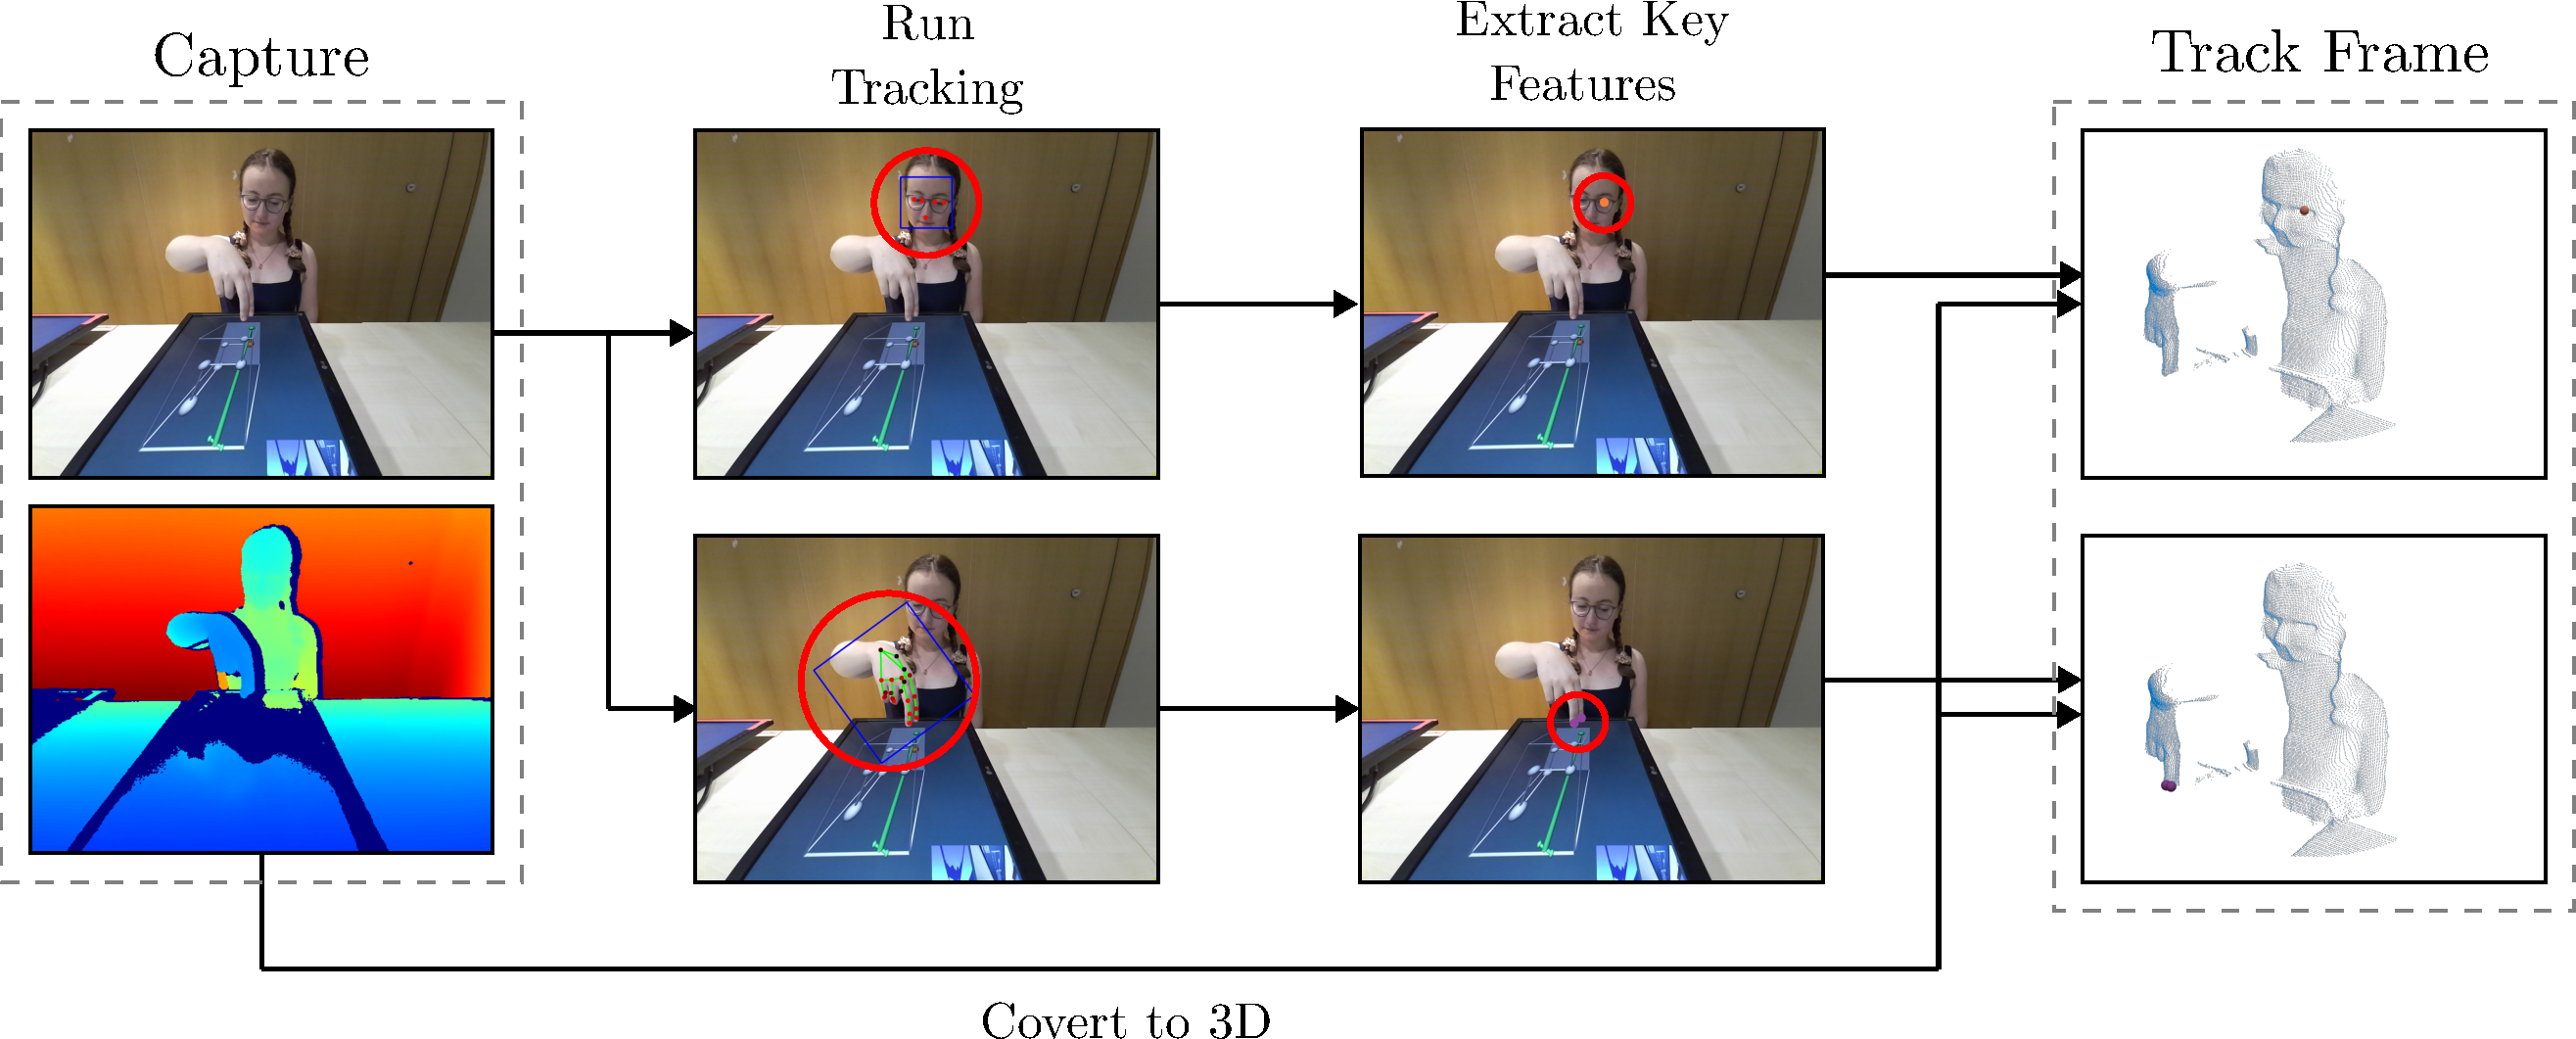
\includegraphics[width=1.0\linewidth]{./implementation/figures/tracker.pdf}
\end{figureBox}

As illustrated in Fig~\ref{fig:tracker-overview}, the process flow of the tracking system is as follows:

\begin{enumerate}[itemsep=-0.25em]
    \item \textbf{Retrieve Capture:} The Kinect Camera is polled to receive a capture.
    \item \textbf{Run Tracking:} Hand and head tracking are performed on the colour image.
    \item \textbf{Extract Key Features:} The positions of the tracked points are extracted from the hands (middle and index fingertips) and face (left eye).
    \item \textbf{Convert to 3D:} The depth image is sampled to convert the 2D points into 3D points, which are then placed in a "tracking frame" to be sent to the renderer.
\end{enumerate}

While it might seem unconventional, we maintain separate instances for tracking the left eye and the thumb and index fingertips. This approach is necessary because there is no guarantee that the tracker will detect both the face and hands in a single pass through. For instance, if the user holds their hand in front of their face, the tracker may only detect the hand. Additionally, there is a possibility that either of the tracking models may fail to detect the intended features. In such cases, our system will reuse the last known position and the corresponding capture, which serves as a reasonable approximation for the eye or finger positions. This strategy also helps to reduce the jerkiness effect that can occur with sporadic dropouts. \\

It is important to note that, for performance reasons, we do not calculate the 3D positioning of the points until the renderer requests them. This approach minimises resource wastage. If we can process a capture faster than the renderer can render a frame, we only calculate the 3D positioning for the most recent capture.

\subsection{Tracking Models}

\subsubsection{Dlib}
We use Dlib to track the left eye's position through a two-stage process. In the first stage, we utilise a Max-Margin Object Detection model \cite{king2015maxmargin, noauthor_dlib_nodate} implemented with a convolutional neural network (CNN) \cite{DBLP:journals/corr/Schmidhuber14}. Instead of training our own model, we used a pre-trained model provided by Dlib \cite{noauthor_index_nodate}, known as \texttt{mmod\_human\_face\_detector}. Initially, we ran the face detection model on the CPU; however, this created a bottleneck in our tracking pipeline. Therefore, we opted to run our CNN on a GPU using CUDA-accelerated functions to meet our performance requirements. \\

Once the user's face is detected, we proceed to the second stage of our facial landmark detection model. We chose to use a five-landmark pose estimator called \texttt{shape\_predictor\_5\_face\_landmark}, leveraging Dlib's implementation of a method proposed in "One Millisecond Face Alignment with an Ensemble of Regression Trees" \cite{6909637}, trained on the iBUG 300-W face landmark dataset \cite{6755925}. This pose estimator operates efficiently enough on a CPU, so GPU acceleration was unnecessary. \\

An example of the results obtained from running the two Dlib models can be seen in Fig~\ref{fig:face-tracker}.

\begin{invisBox}
    \pictureBox[label={fig:face-tracker}]{Dlib Face Tracker}{
        \adjustbox{height=5.75cm, keepaspectratio}{
            \includegraphics{./implementation/figures/Face-tracker.png}
        }
    }
    \hfill
    \pictureBox[label={fig:hand-tracker}]{MediaPipe Hand Tracker}{
        \adjustbox{height=5.75cm, keepaspectratio}{
            \includegraphics{./implementation/figures/hand-tracker.png}
        }
    }
\end{invisBox}

\subsubsection{MediaPipe}
We use MediaPipe to track the position of two fingers on the user's hand, employing a two-stage process. MediaPipe uses a two-stage model to track hands \cite{zhang2020mediapipe}. The first stage involves a palm detection model that identifies the position of the hand within the image. The second stage is a hand landmark model that detects the positions of 21 points on the hand. MediaPipe provides an interface that allows us to feed images as a stream, abstracting away most of the detection logic, unlike Dlib. \\

We chose to track the positions of the index and middle fingers because this configuration proved to be more stable than tracking the thumb and index finger, and it led to fewer instances of accidental occlusion. To enhance the tracking accuracy, we depth-sample from the surface of the hand and apply a constant offset to make it appear as though the point is inside the hand. An example of the results from running the two MediaPipe models can be seen in Fig~\ref{fig:hand-tracker}.

\subsubsection*{Downscaling}
To ensure that our tracking system operates at a sufficient frame rate, we downscale the images obtained from the camera. We found that downscaling the images using an image pyramid \cite{adelson1984pmi} by a factor of 2 still yields accurate tracking results. This significantly improves the performance of our tracking system. Further details can be found in the evaluation section.

%%%%%%%%%%%%%%%%%%%%%%%%%%%%%%%%%%%%%%%%%%%%%%%%%%%%%%%%%%%%%%%%%%%%%%%%%%%%%%%%%%%%%%%%%%%%

\subsection{Multithreading}

One of the more challenging aspects of this project was making our tracking system performant enough to feel smooth and responsive. To achieve this, we implemented a multi-threaded design, as outlined in Fig~\ref{fig:mult-threaded-des}. We used separate threads for tracking, capturing, and rendering.

\begin{figureBox}[label={fig:mult-threaded-des}, width=0.75\linewidth]{Multi-threaded Design}
    \includegraphics[width=1.0\linewidth]{./implementation/figures/multi-thread-design.pdf}
\end{figureBox}

The purpose of this design was to ensure that the tracking thread and models were utilised 100\% of the time, as they are the most computationally intensive components of the system and represent the main bottleneck. While using a multithreaded design does not reduce the system's latency (as discussed further in the evaluation section), it significantly increases the application's throughput and frame rate.

\begin{figureBox}[label={fig:single-vs-multi}, width=0.75\linewidth]{Single vs Multi-threaded Design}
    \includegraphics[width=0.8\linewidth]{./implementation/figures/single-vs-multi.pdf}
\end{figureBox}

Since the Kinect camera operates at 30 fps, we need to process an image every $ \frac{1000 \text{ ms}}{30} = 33.3 \text{ ms}$ to ensure that we handle every frame. In our initial single-threaded implementation, we were unable to achieve this rate. By switching to a multi-threaded design, we decreased the time required to produce a new tracking frame to match the duration of the slowest thread (the tracker thread), as shown in Fig~\ref{fig:single-vs-multi}. This also allowed us to run the simulation at a frame rate independent of the tracker. Although this design resulted in the capture thread often being idle, the overall system was light on resources, making this trade-off worthwhile for the significant frame rate improvement it provided.

%%%%%%%%%%%%%%%%%%%%%%%%%%%%%%%%%%%%%%%%%%%%%%%%%%%%%%%%%%%%%%%%%%%%%%%%%%%%%%%%%%%%%%%%%%%%

\subsection{GPU Acceleration}

Another method we utilised to enhance the performance of our tracking system is GPU/CUDA acceleration. Both Dlib and MediaPipe support GPU acceleration. However, we only needed to use GPU acceleration in Dlib because the CPU speed was already sufficient for our tracking pipeline in MediaPipe. The reported speedup of 12.27 ms with GPU acceleration versus 17.12 ms without \cite{noauthor_hand_nodate} did not justify the effort required to enable CUDA in MediaPipe, especially given the complexities involved in building with Nix (see the build systems section for more information). \\

As illustrated in Fig~\ref{fig:system-des}, we only used GPU acceleration for two parts of our tracking system, excluding rendering. We utilised OpenCV's GPU-accelerated pyramid down function to downscale our colour images, as this task is highly parallel and benefits significantly from acceleration. Additionally, we executed the Dlib CNN for face detection on the GPU.

\begin{figureBox}[label={fig:system-des}, width=0.95\linewidth]{Overall Tracking System Design}
    \includegraphics[width=1.0\linewidth]{./implementation/figures/tracking-system.pdf}
\end{figureBox}

%%%%%%%%%%%%%%%%%%%%%%%%%%%%%%%%%%%%%%%%%%%%%%%%%%%%%%%%%%%%%%%%%%%%%%%%%%%%%%%%%%%%%%%%%%%%

\subsection{Camera Positioning}

To ensure that the tracking system is calibrated correctly and that the user sees the correct perspective, it is crucial to know the relative position of the camera to the screen. Misalignment can lead to a distorted and incorrect user experience, where objects will appear to be in the wrong location/orientation relative to the user's point of view. An example of correct and incorrect calibration can be seen in Fig~\ref{fig:calibration}. We developed a calibration system to automate the process of determining accurate position and orientation values. The calibration system operates as follows:
\begin{enumerate}[itemsep=-0.3em]
    \item The camera and displays' position and orientation are measured in 3D space.
    \item The relative positions of the camera and screen are input into the system.
    \item The predicted position of the screen is rendered in 3D.
    \item The predicted position of the screen is iteratively adjusted until it aligns with the true position.
\end{enumerate}

\begin{figureBox}[label={fig:calibration}, width=0.65\linewidth]{Display Calibration}
    \includegraphics[width=1.0\linewidth]{./implementation/figures/calibration.pdf}
\end{figureBox}


\label{sect:tracker}
\section{User Study}
\begin{enumerate}
	\item Use Image from plan.
	\item Horizontal Monitor on side. 
\end{enumerate}
\label{sect:userstudy}

% %%%%%%%%%%%%%%%%%%%%%%%%%%%%%%%%%%%%
\chapter{Evaluation}
\section{Simulator Evaluation}
\begin{enumerate}
	\item Measure Latency
	\item Measure Accuracy (How often tracker loses track of hand)
\end{enumerate} 
\label{sect:eval-volsim}
\section{User Study}
\begin{enumerate}
	\item Use Image from plan.
	\item Horizontal Monitor on side. 
\end{enumerate}
\label{sect:eval-userstudy}

%%%%%%%%%%%%%%%%%%%%%%%%%%%%%%%%%%%%
\chapter{Future Work, Conclusions and Contributions}
\section{Future Work}

We have identified several areas for future work that could enhance the capabilities and usability of our volumetric display simulator and further explore the potential of volumetric displays in interactive 3D applications.

\subsection{Anaglyph 3D}
Anaglyph 3D \cite{Dhaou2019} is a technique for displaying 3D images using colour-filtered glasses, typically employing red and green filters. Unlike polarized 3D \cite{article-3D}, it does not require additional complex hardware. Currently, the 3D effect necessitates closing one eye. Integrating 3D support into the system could enhance the immersive experience by eliminating this limitation.

\subsection{Multi-User Support}
Another potential area for future exploration is multi-user support. Our current tracking system is limited to a single user. Extending it to support multiple users would be a logical progression and relatively straightforward. By utilizing colour filter glasses or shutter glasses, it is feasible to render different perspectives to multiple users simultaneously, as suggested in the study "Two Kinds of Novel Multi-user Immersive Display Systems" \cite{Two-Kinds}.

\subsection{Real-Time Light Detection}
Adding an additional camera with a fisheye lens to generate a real-time light map could be a valuable enhancement. This feature would enable the virtual scene to be illuminated by real-world lighting conditions. It would be insightful to investigate whether this addition impacts performance in any significant way, especially concerning the tasks evaluated in our user study.

\subsection{Generalize CPU/GPU Camera Compatibility}
The current project is compatible only with Nvidia GPUs. Expanding compatibility to include AMD GPUs, Intel GPUs, and even CPU-only environments (with expected slower performance) would be beneficial. Furthermore, supporting different depth cameras beyond the Kinect, such as Intel RealSense Depth Cameras \cite{keselman2017intel}, is crucial, particularly since the Kinect has been discontinued by Microsoft. Achieving this will require substantial code generalization. Switching cameras to a lower latency system would also be beneficial.

\subsection{Switch Hand Tracking Model}
The hand tracking component of the project is notably the weakest aspect. Transitioning to a more robust hand tracking model is highly recommended. Specifically, adopting a model that utilises depth images rather than RGB images could significantly improve performance. This would likely be a major undertaking, as off-the-shelf models for this purpose are scarce. Implementing the approach described in the paper "Accurate, Robust, and Flexible Real-Time Hand Tracking" \cite{sharp2015accurate} appears promising.

\subsection{Further User Study}
As indicated in the evaluation section, while the user study provided conclusive results, further investigation is warranted. We are interested in exploring various offset positions to examine the drop-off rate in greater detail. Additionally, adjusting the position of the interaction zone, as opposed to the display position, could yield valuable insights.

\subsection{Porting to Windows and Mac}
Although we have demonstrated that the project can be built with a single command on Linux, extending support to Windows (including WSL) and Mac would be advantageous. We have successfully compiled the project on Windows, but further investigation is required to address WSL-specific issues. We have yet to attempt building it on Mac. This is expected to be more challenging, as porting all GPU-accelerated functionality to Apple Metal \cite{noauthor_httpsdeveloperapplecommetalmetal-shading-language-specificationpdf_nodate} may pose significant difficulties, despite Nix's native compatibility with Mac.

\section{Conclusions}

The development and evaluation of our Volumetric Display Simulator underscore its potential as a versatile tool for future research in volumetric display technologies. By integrating cost-effective components and reproducible software environments, we have created a system that is both accessible and straightforward, encouraging wider adoption and further development by other researchers. \\

Our user study demonstrated that the use of head tracking and direct hand interaction significantly enhances task performance in a 3D environment, highlighting the importance of natural interaction modes for effective use of volumetric displays. The findings suggest promising avenues for future research, including the exploration of positional offsets and interaction zone dynamics, which could lead to significant improvements in the usability and functionality of volumetric displays.
\label{sect:conclusions}

%%%%%%%%%%%%%%%%%%%%%%%%%%%%%%%%%%%%
\printbibliography

\appendix
\chapter{Final Package}
\label{app:final-package}
\section{VolumetricSim Package}
The result of building our simulator is a shared library named \texttt{libvolsim.so} shown in Listing~\ref{list:libvolsim}.
\codeBoxFile[label = {list:libvolsim}]{shell}{./implementation/code/libvolsim.sh}{Terminal}
\chapter{Survey Forms}
\label{app:survey}
\section{Form A: Overall Digital Survey Form}
This form is the primary survey that was given to participants in the user study. It was used to collect data on the participants' demographics, their experience with technology, and their opinions on the volumetric display system.


\includepdf[pages=-]{./appendix/files/Volumetric Display User Study.pdf}
\section{Form B: Inter-Condition Survey Form}
This was the phyiscal survey that was given to participants in the user study. It was used to collect data on the participants' opinions between the different conditions of the volumetric display system. The results were copied into a digital form. 

\includepdf[pages=-]{./appendix/files/Document For User Study.pdf}
\chapter{Extended User Study Results}
\label{app:results}
\section{Comprehensive Results}
Presented below are the detailed graphs and results from our user study, organized on a task-by-task basis. The graphs are divided into five sections, each corresponding to a specific task. The first two graphs are similar to those found in Evaluation~\ref{sect:eval-userstudy}, but are applied exclusively to this task. The subsequent four graphs display the fully plotted 3D paths of users under each condition, with each segment represented in a distinct color.

\newpage
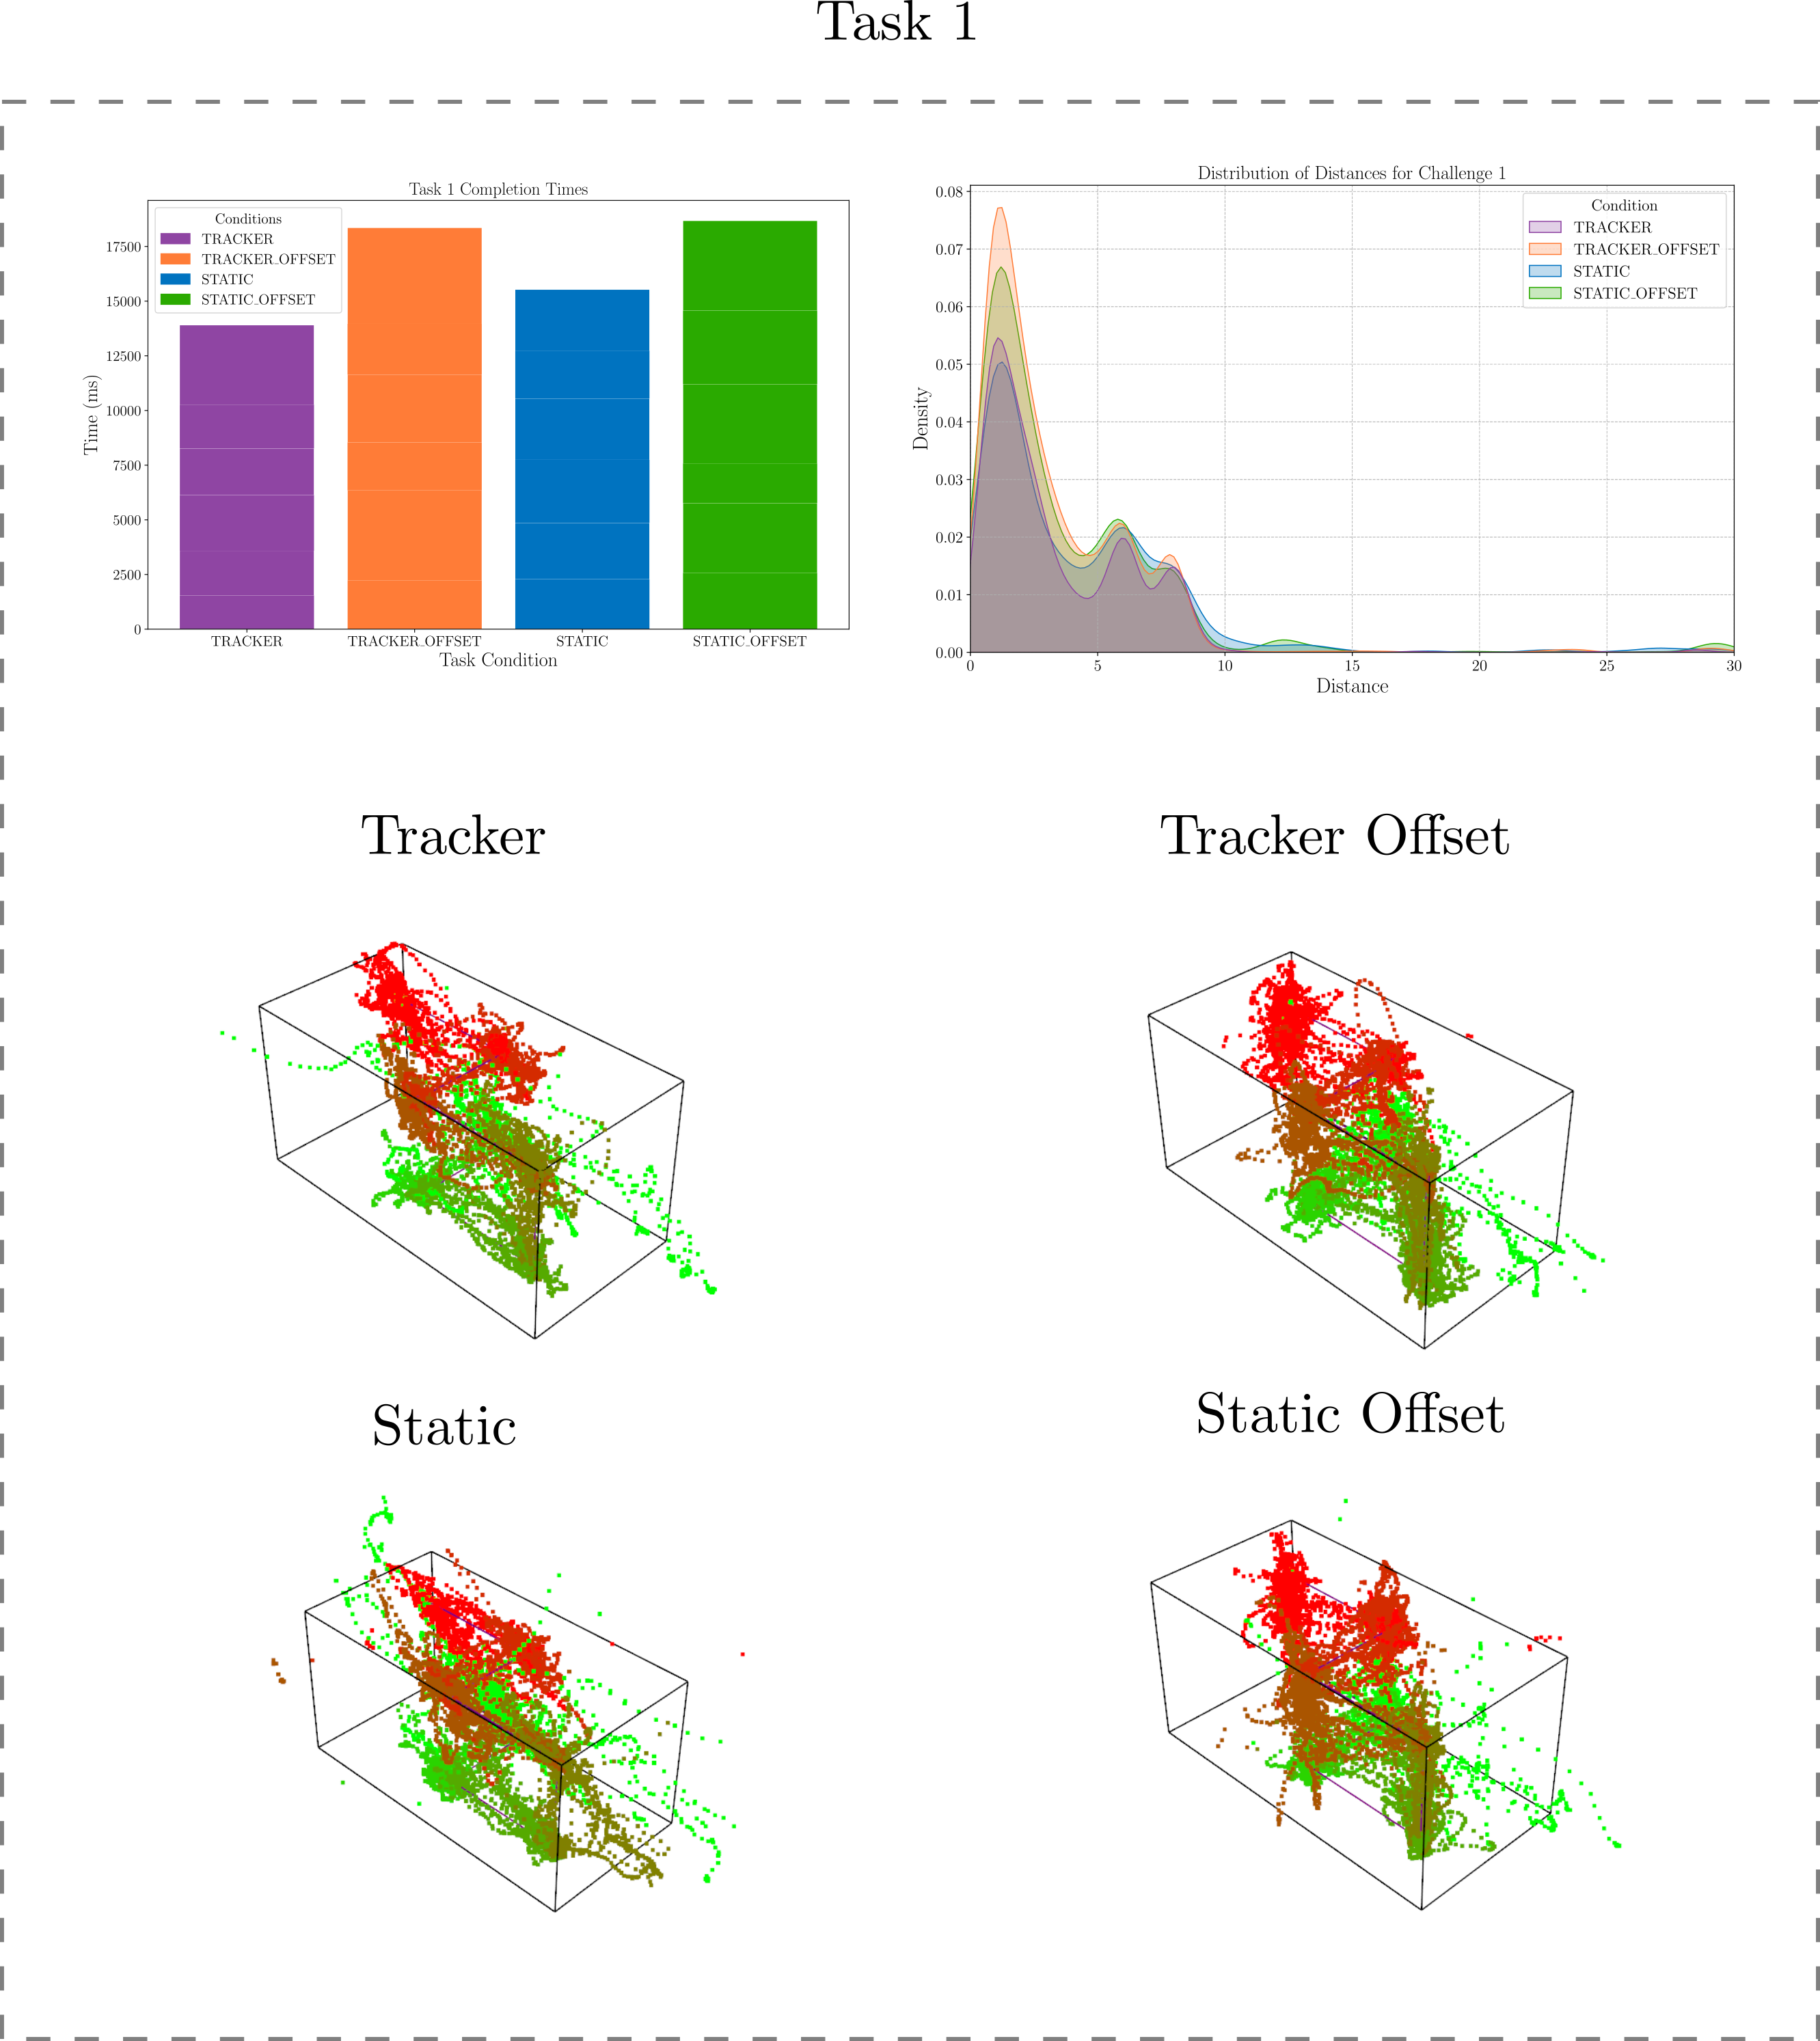
\includegraphics[scale=0.8]{./appendix/files/graphs-1.png}
\newpage
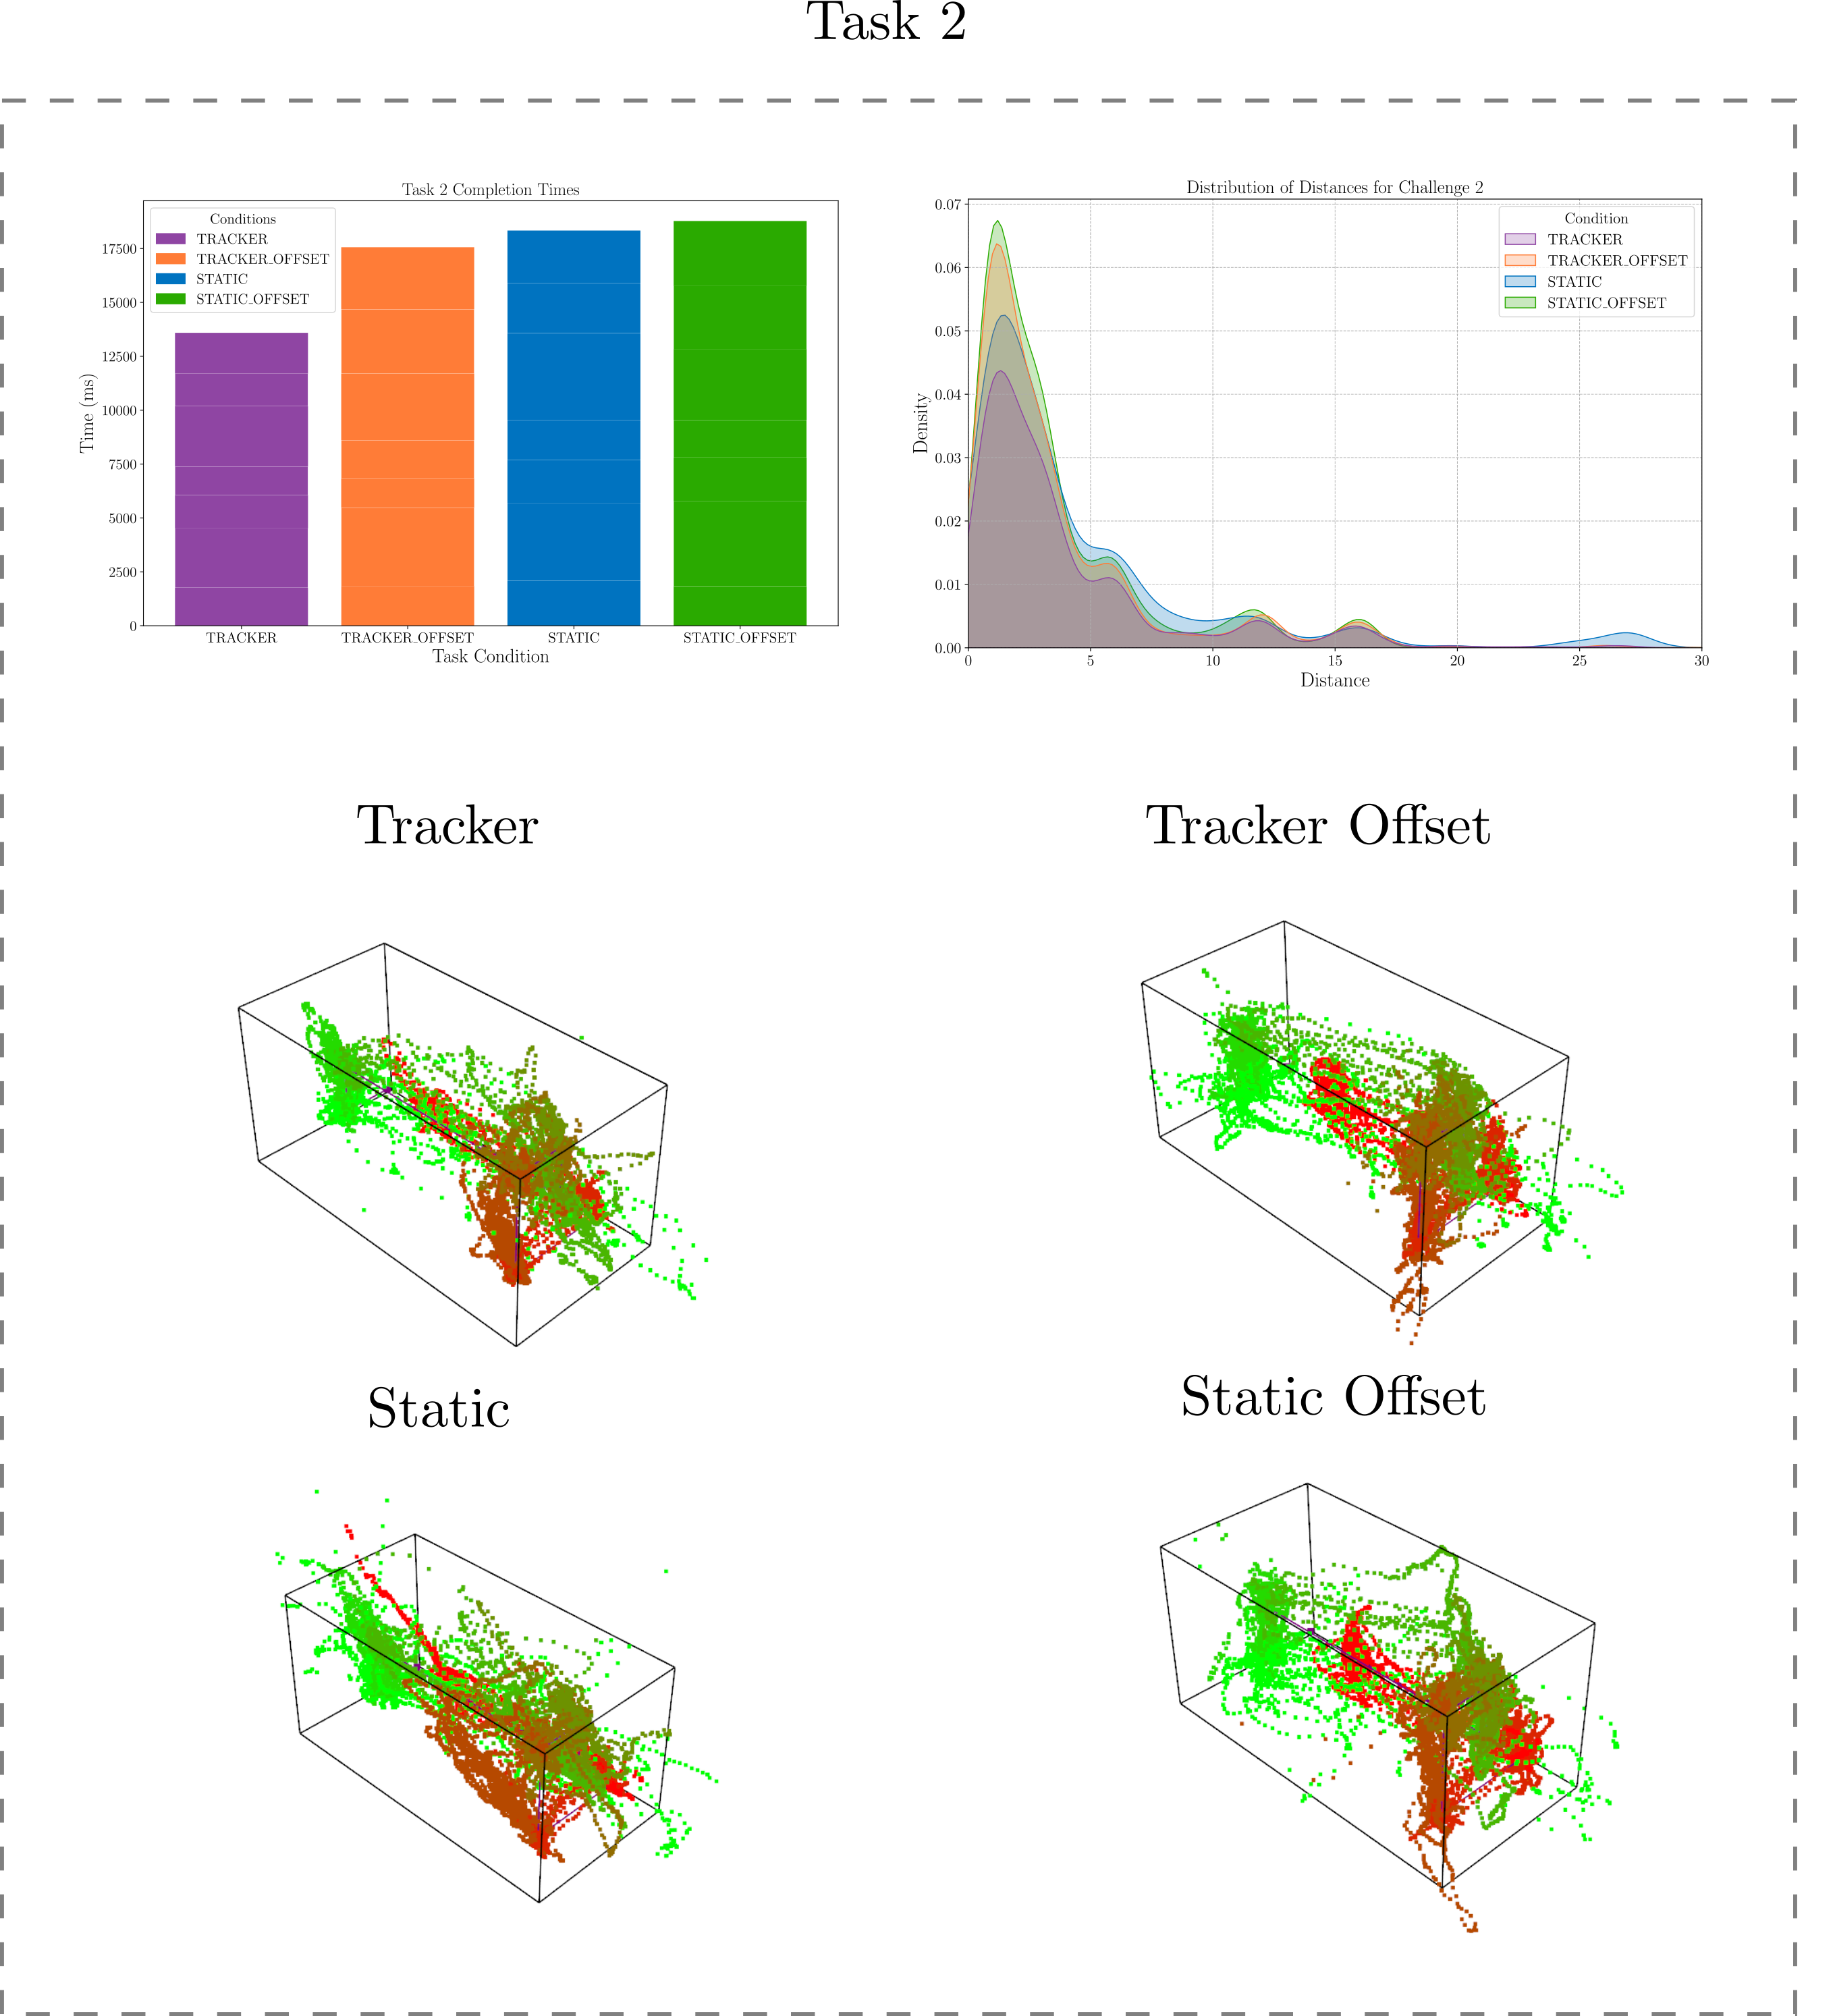
\includegraphics[scale=0.8]{./appendix/files/graphs-2.png}
\newpage
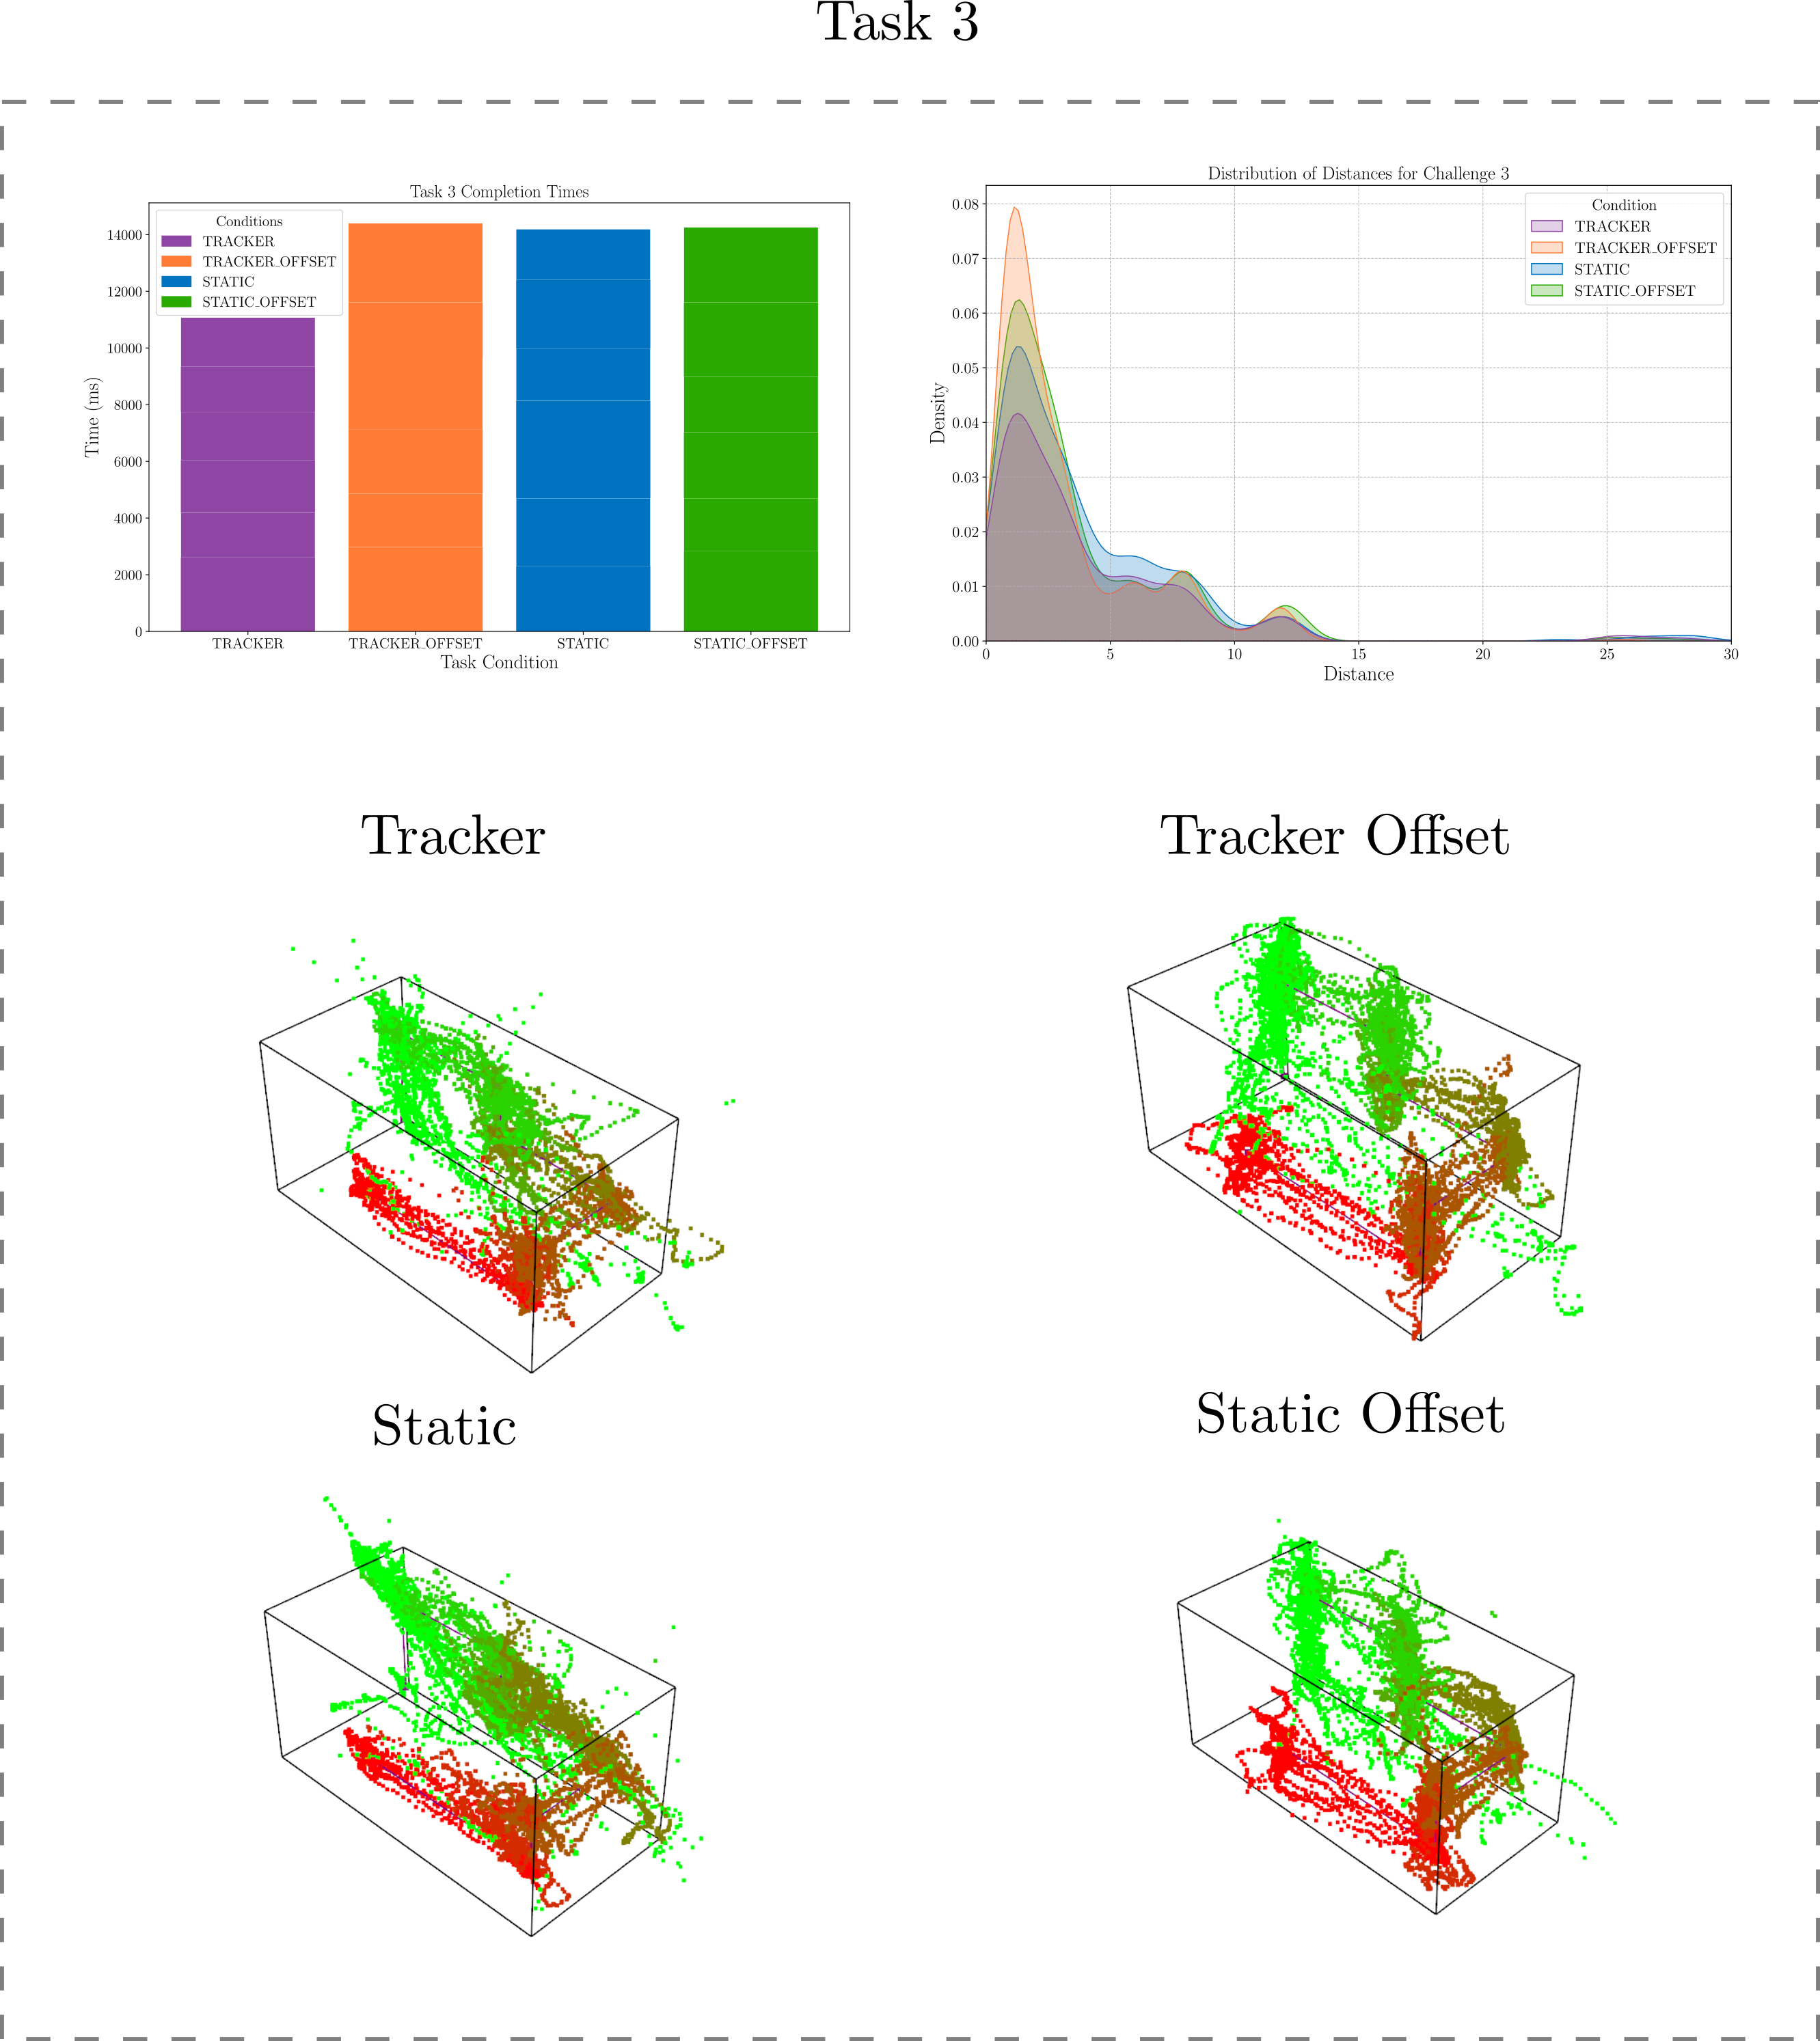
\includegraphics[scale=0.8]{./appendix/files/graphs-3.png}
\newpage
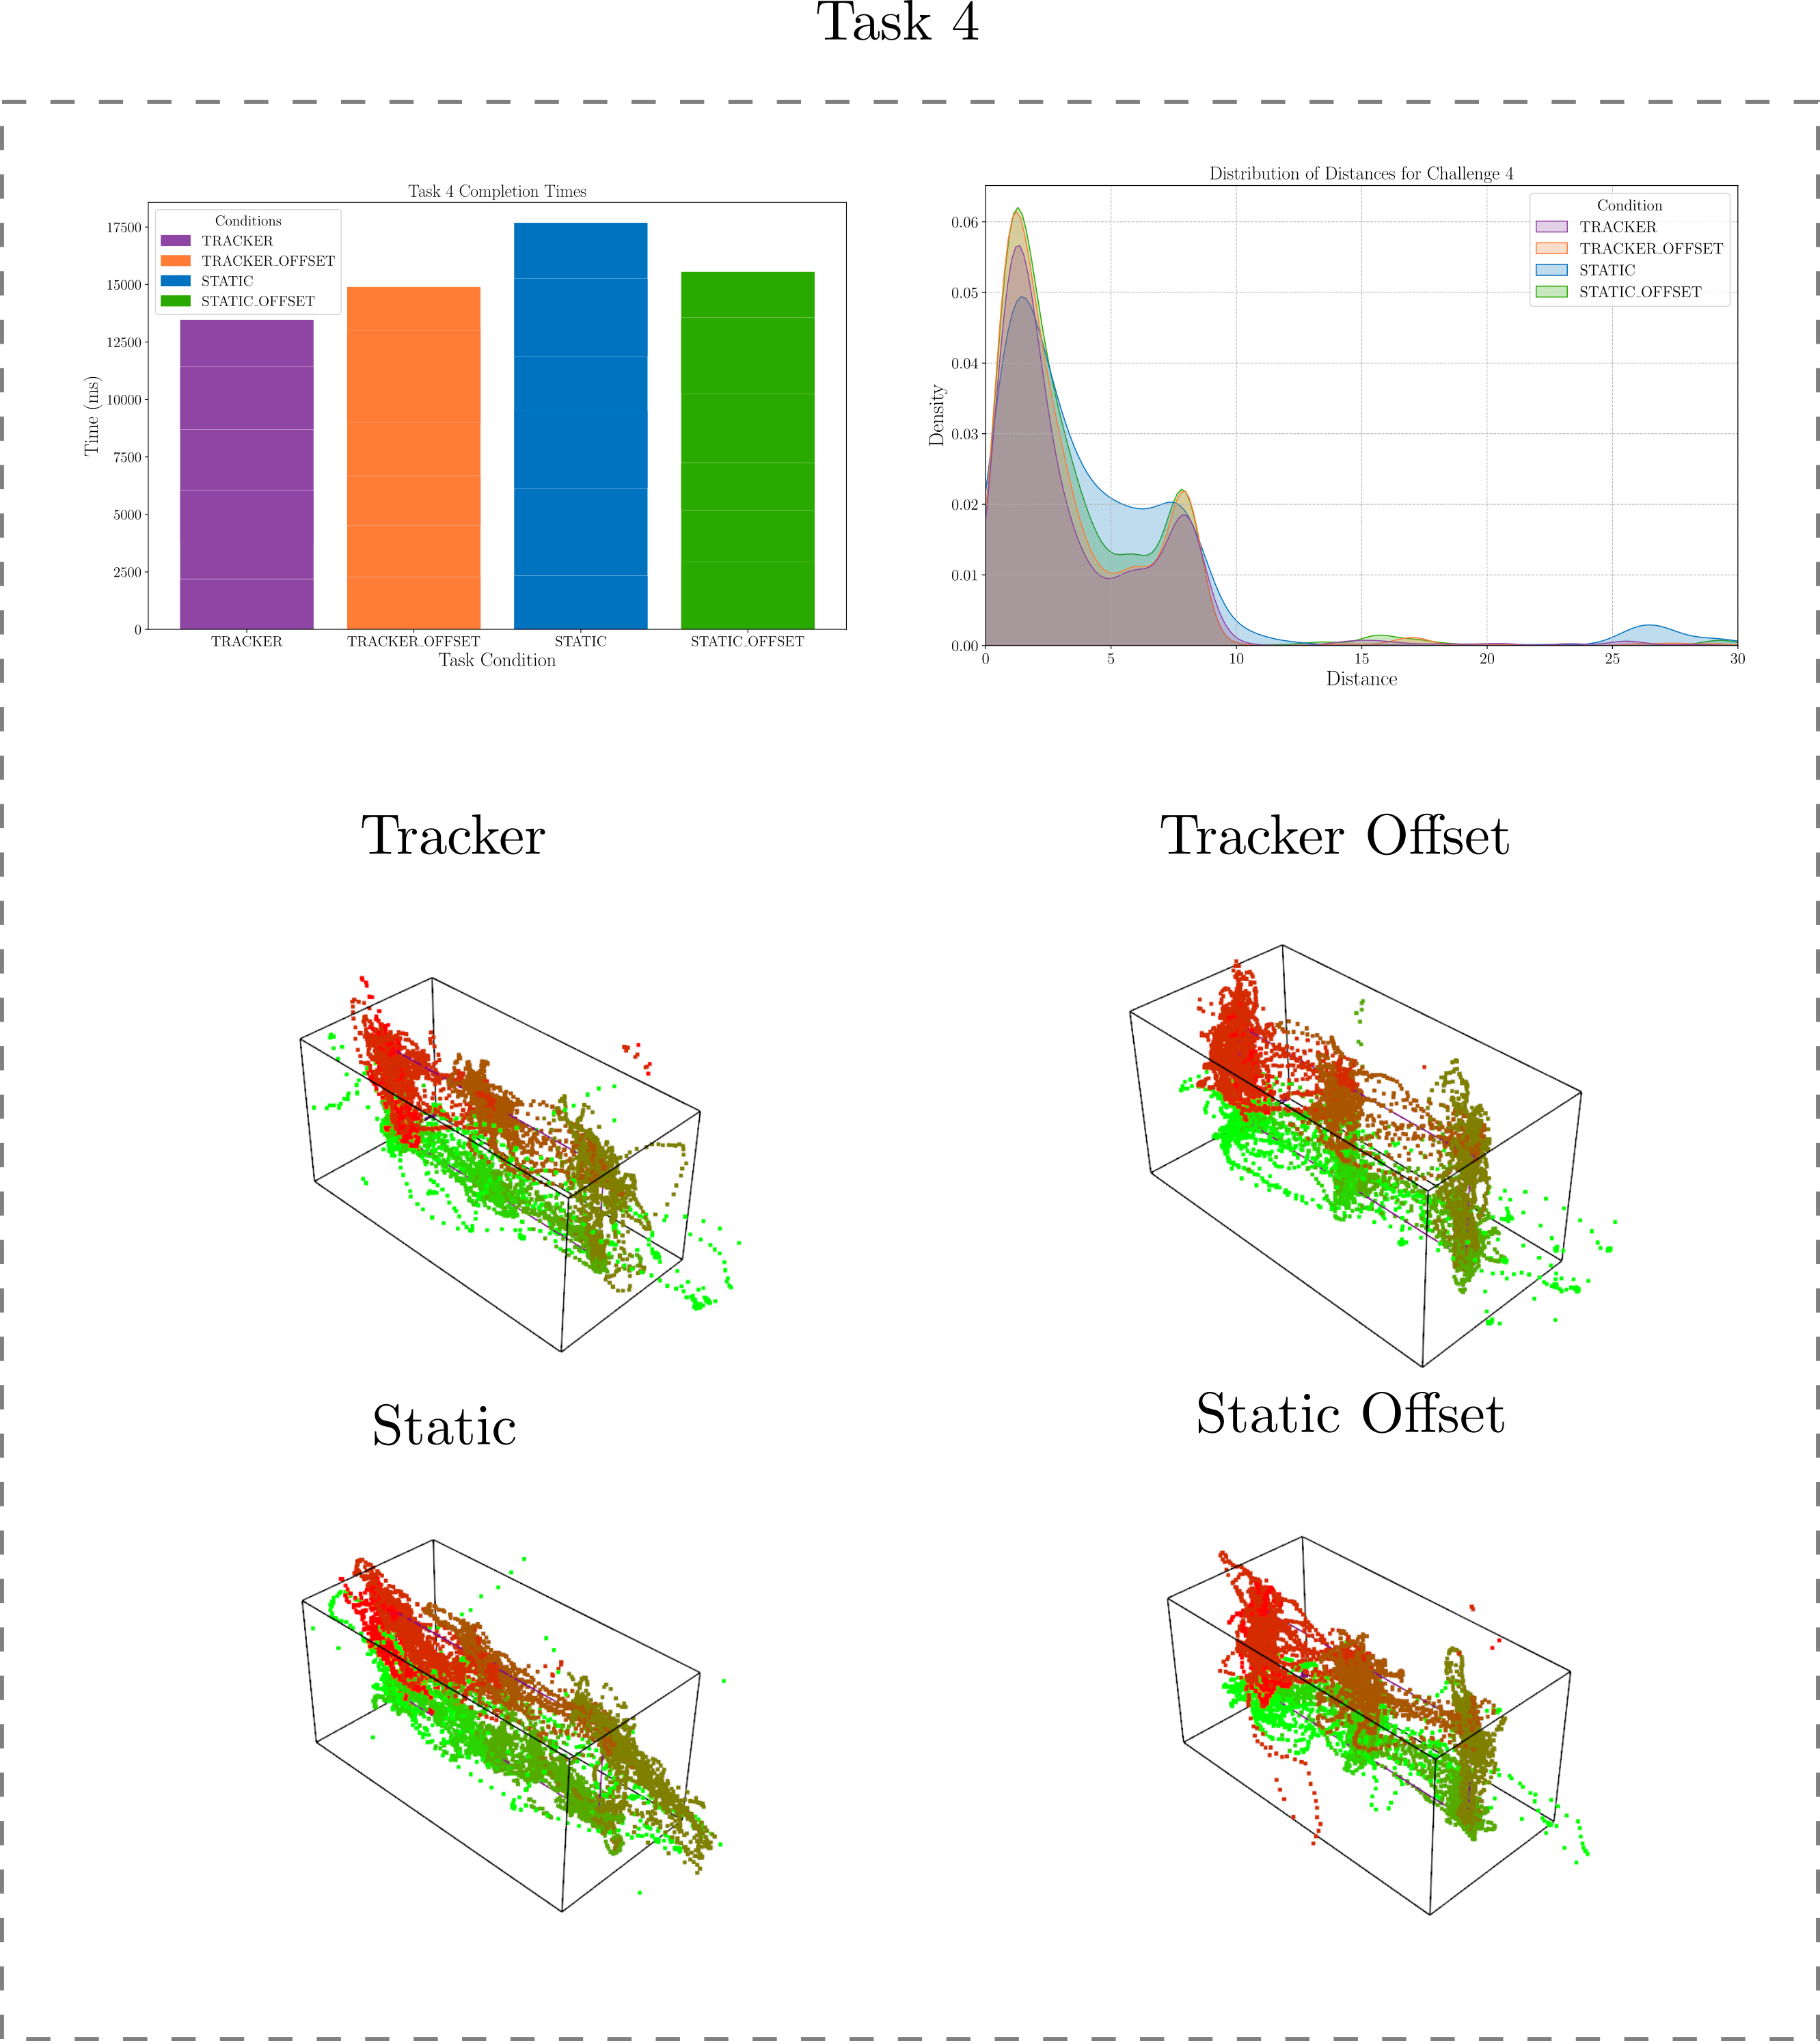
\includegraphics[scale=0.8]{./appendix/files/graphs-4.png}
\newpage
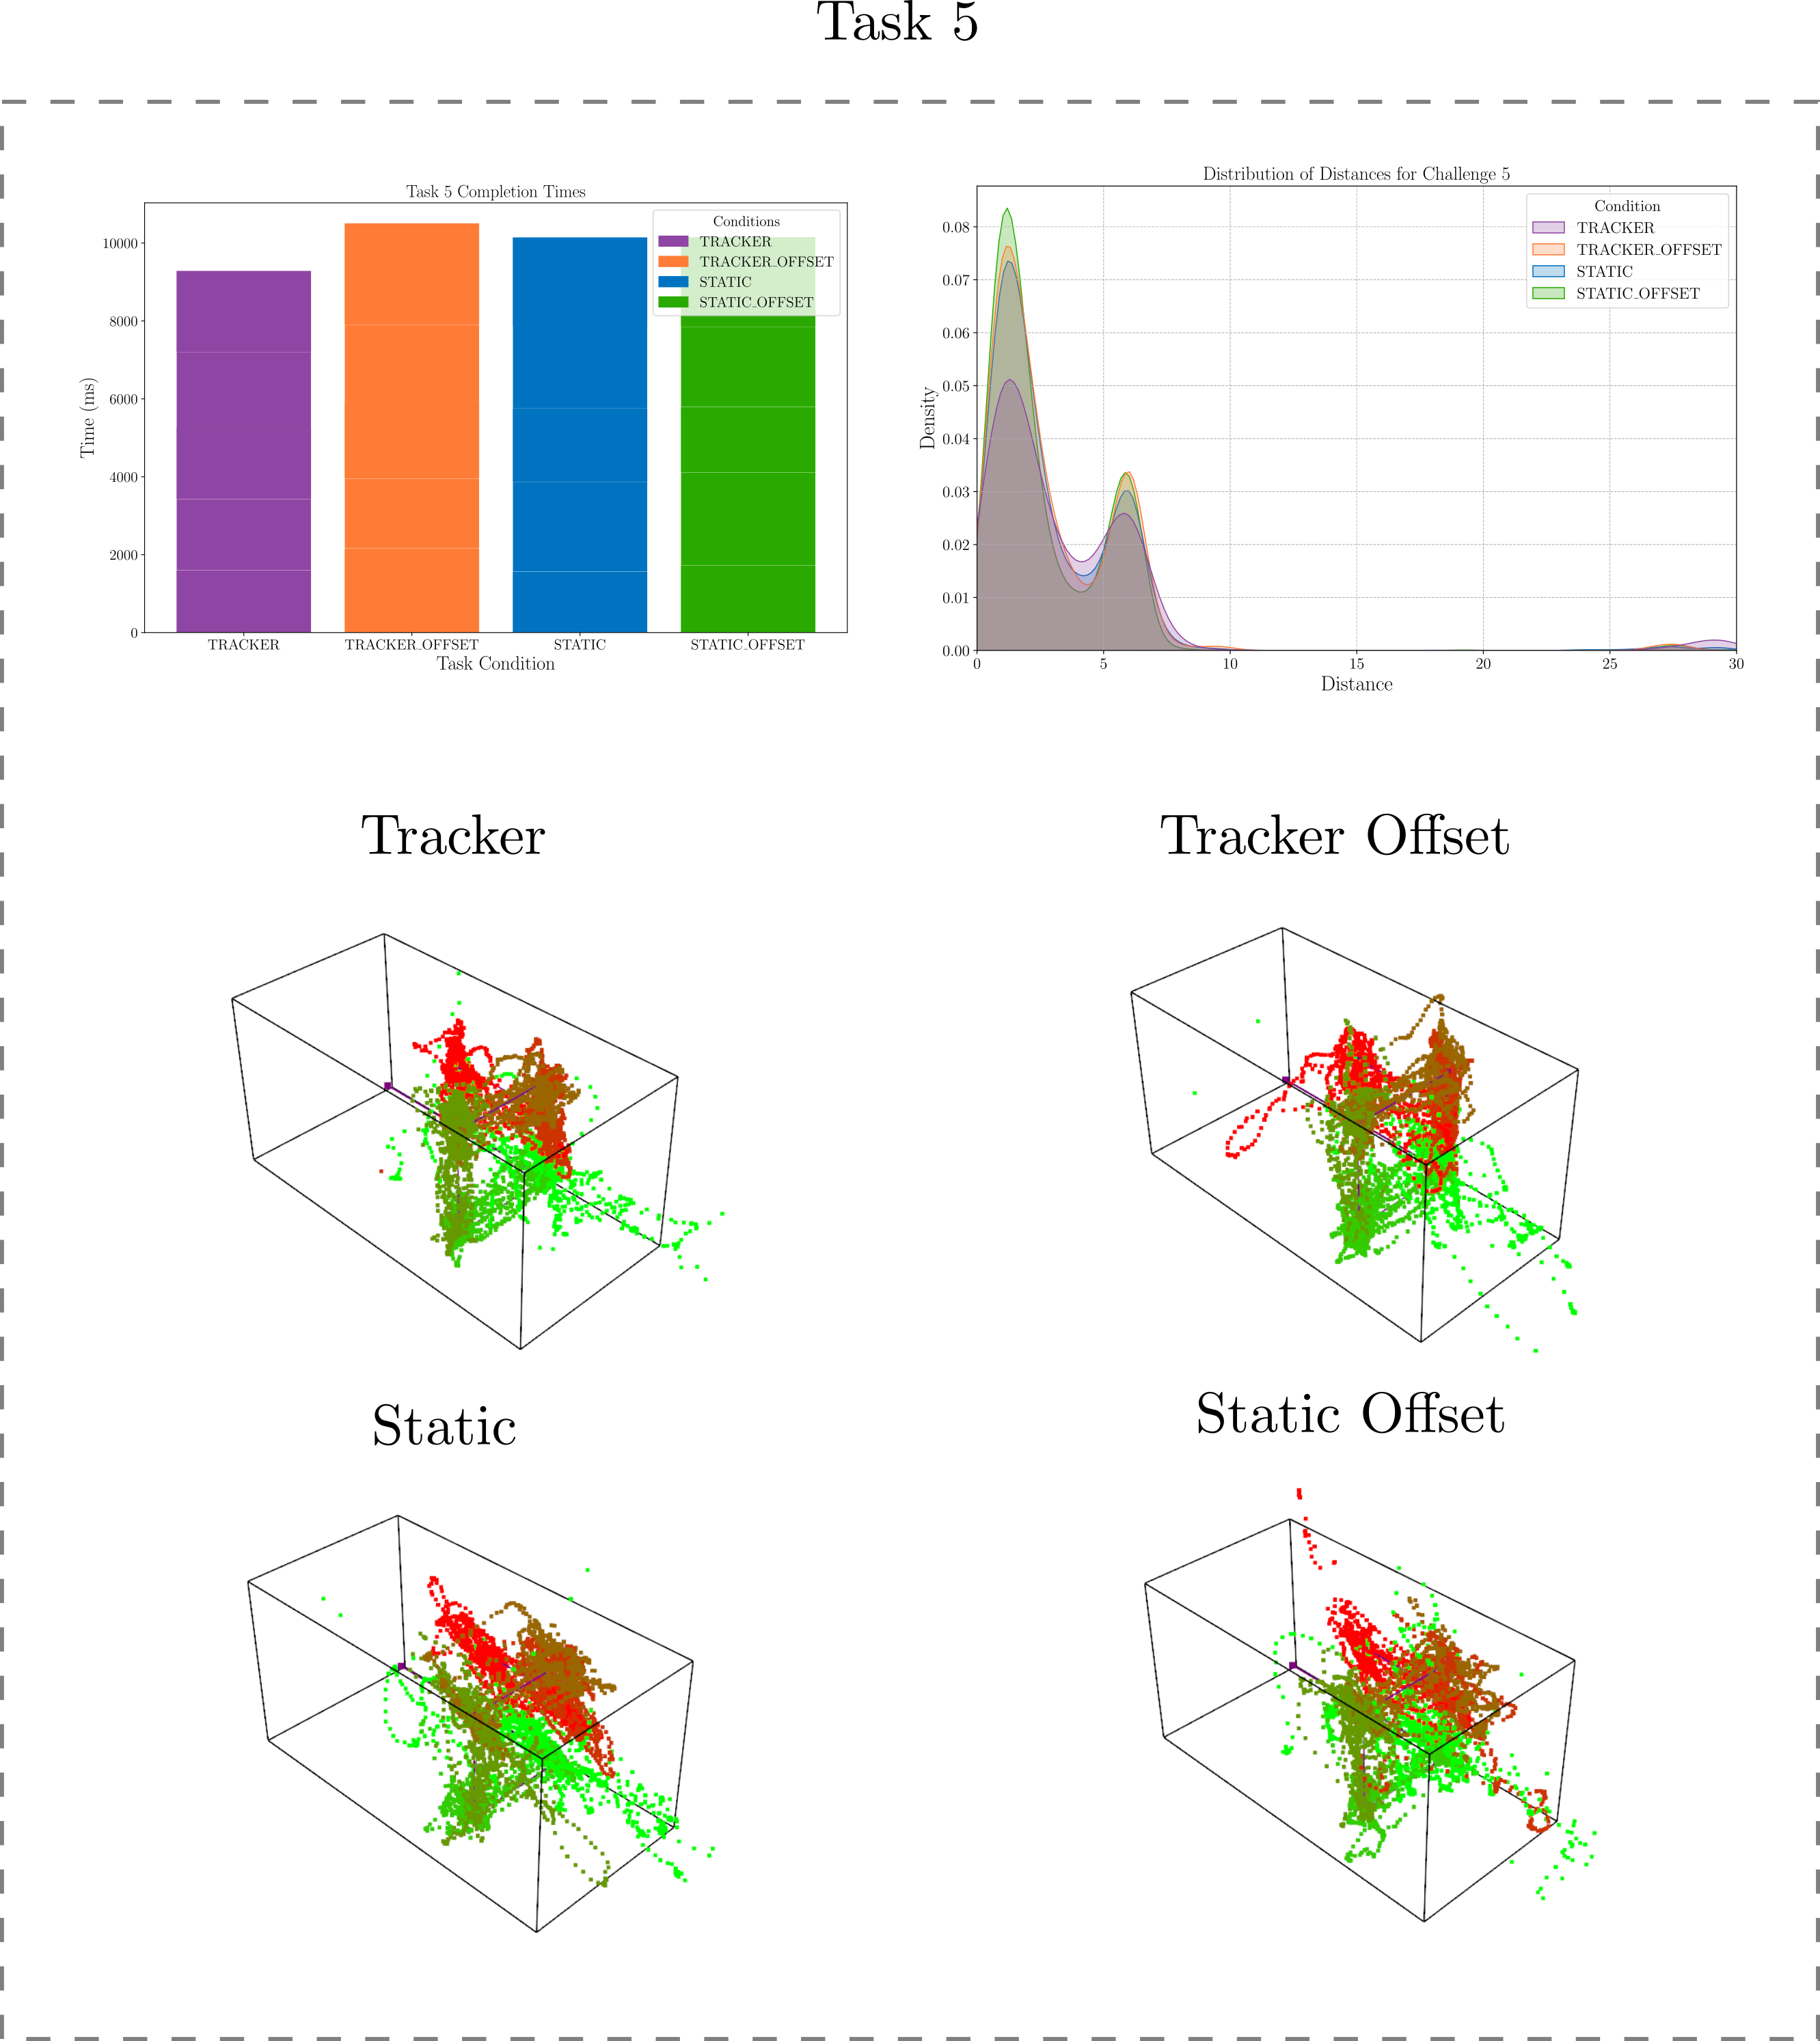
\includegraphics[scale=0.8]{./appendix/files/graphs-5.png}

\end{document}